%%%%%%%%%%%%%%%%%%%%%%%%%%%%%%%%%
%Preamble
%%%%%%%%%%%%%%%%%%%%%%%%%%%%%%%%%

\PassOptionsToPackage{usenames, dvipsnames}{xcolor}

\documentclass[a4paper, table]{article}
\usepackage[english]{babel}
\usepackage[margin=1in]{geometry}
\usepackage[ruled, vlined]{algorithm2e}

\usepackage{amsfonts}
\usepackage{setspace,graphicx,epstopdf,amsmath}
\usepackage{marginnote, datetime, url, enumitem, subfigure}

%Journal Style
%JFE looks nice, JF looks awful
	\usepackage{amsthm}
	\usepackage{jfe}

%Bibliography Stuff
	%Use natbib even though it's old because it's compliant with journal styles
	%Actual bibliography style etc are specified where you actually want it
	\usepackage{natbib}

%Fluff
	\linespread{1.3}

%Neural Network Packages
	\usepackage{neuralnetwork}
	\usepackage{xpatch}
	\makeatletter
	% \linklayers have \nn@lastnode instead of \lastnode,
	% patch it to replace the former with the latter, and similar for thisnode
	\xpatchcmd{\linklayers}{\nn@lastnode}{\lastnode}{}{}
	\xpatchcmd{\linklayers}{\nn@thisnode}{\thisnode}{}{}
	\makeatother
	
%Regression Tree
	\usepackage{tikz,forest}
	\usetikzlibrary{arrows.meta}
	
	\forestset{
		.style={
			for tree={
				base=bottom,
				child anchor=north,
				align=center,
				s sep+=1cm,
				straight edge/.style={
					edge path={\noexpand\path[\forestoption{edge},thick,-{Latex}] 
						(!u.parent anchor) -- (.child anchor);}
				},
				if n children={0}
				{tier=word, draw, thick, rectangle}
				{draw, diamond, thick, aspect=2},
				if n=1{%
					edge path={\noexpand\path[\forestoption{edge},thick,-{Latex}] 
						(!u.parent anchor) -| (.child anchor) node[pos=.2, above] {Y};}
				}{
					edge path={\noexpand\path[\forestoption{edge},thick,-{Latex}] 
						(!u.parent anchor) -| (.child anchor) node[pos=.2, above] {N};}
				}
			}
		}
	}

\usepackage{lscape}
\usepackage{longtable}

%%TODONOTE commands
\usepackage[colorinlistoftodos]{todonotes}
\newcommand{\smalltodo}[2][] {\todo[caption={#2}, size=\scriptsize,%
	fancyline,#1]{\begin{spacing}{.5}#2\end{spacing}}}
\newcommand{\rhs}[2][]{\smalltodo[color=green!30,#1]{{\bf RS:} #2}}
%%

%Graphs
\usepackage{tikz}
\usepackage{pgfplots}
\graphicspath{{../Results/}}

%Coloured Tables

%%%%%%%%%%%%%%%%%%%%%%%%%%%%%%
%%Title and other fluff, just before document start
%%%%%%%%%%%%%%%%%%%%%%%%%%%%%%

%Hyperref apparently is a big package and causes a lot of issues, so it's recommended to load this last

\usepackage{hyperref}

%Gets rid of the neon green boxes around boxes

\usepackage[]{xcolor}

\hypersetup{
	colorlinks,
	linkcolor = {red!50!black},
	citecolor = {blue!50!black},
	urlcolor = {blue!80!black}
}

\title{Evaluation of Machine Learning in Empirical Asset Pricing}
\author{Ze Yu Zhong}

%%%%%%%%%%%%%%%%%%%%%%%%%%%%%%%
%%BEGIN DOCUMENT
%%%%%%%%%%%%%%%%%%%%%%%%%%%%%%%

\begin{document}

\maketitle

\tableofcontents

\newpage

%%%%%%%%%%%%%%%%%%%%%%%%%%%%%%%%%%%%%%%%%%%%%%%%%%%%%%%%%%%%%%%%%%%%%%%%%%%%%%%%%%%%%%%%%%%%%%%%%%%%%

\section{Introduction}

\subsection{Topic}

This thesis aims to evaluate the application of machine learning algorithms in empirical asset pricing. While there has been significant recent interest in applying machine learning to the problem of predicting asset returns, there is little literature that focuses on how well these algorithms are at capturing true underlying variables in determining stock returns. 12 different simulated datasets ranging from linear to highly non-linear data generating processes incorporating observed phenomena of cross sectional correlation, persistence, and stochastic volatility, in addition to real world data will be used to assess the performance of linear models, elastic net models, random forests and neural networks. Model performance will be assessed according to their out of sample Mean Absolute Error, Root Mean Square Error, and Predictive $R^2$, in addition to whether or not they were able to identify the correct variables in the data generating process according to a variable importance metric.

\subsection{Background Literature and Motivations}

This paper is motivated by evaluating the performance of machine learning algorithms in empirical asset pricing, focusing on how well they deal with the many unique problems in financial returns data. Here, we define ``performance" to refer to two forms of metrics conventional in the literature: $R^2$ (and more specifically, out of sample $R^2$), and forecast errors (see \ref{model_evaluation} for more details).

We first begin by defining ``factors" with the more contemporary definition as suggested by \cite{harvey__2016}: a collection of regressors to be used in pricing returns that can be used to proxy for unknown underlying risk factors due to their correlation with cross sectional returns. Most notably, their definition rejects the more strict view that risk factors should be variables that have unpredictable variation through time, and that they should be able explain cross sectional return patterns. \cite{harvey__2016} further groups factors into the two broad categories of ``common" and individual firm ``characteristics." ``Common" factors under this definition can be viewed as proxies for sources of risk constant across all firms, such as macroeconomic variables. Examples of this include the Fama-French factors, which are portfolios of assets sorted by certain characteristics to proxy for them. \cite{harvey__2016} notes that individual firm characteristics are unlikely to satisfy the more strict definition because they are often pre-known and display limited time series variation.

Because of this less strict definition, factors introduced and used in the literature often exhibit properties which makes them unsuitable for inclusion in models, such as high persistence, high levels of non-stationarity and cross sectional correlation. 

\cite{goetzmann_testing_1993} and \cite{ang_stock_2006} note the persistence present in dividend ratio factors. This means that movements in dividend ratios are dominated by movements in price and therefore dividend ratios are correlated with lagged dependent variables on the right hand side of the regression equation. This violates the assumptions of exogeneous regressors (independent from the error term) required for traditional regression models (ordinary least squares) to be unbiased, resulting in t statistics which are biased upwards and increase with time horizon due to autocorrelated errors. Importantly, \cite{goetzmann_testing_1993} show that corrections to t statistics using the Generalized Method of Moments and Newey-West standard errors also appear to be biased upwards, making them unreliable. 

\cite{goyal_predicting_2003} provide a more comprehensive study on the performance of lagged dividend price ratios, with specific focus on out of sample predictive performance both in terms of $R^2$ and forecast errors. They conclude that while models incorporating dividend related factors were able to achieve higher in sample performance prior to 1990 than the historical mean, they could not have outperformed the historical mean \textit{out of sample}. \cite{goyal_predicting_2003} attribute this to the increasing persistence and non-stationarity of dividend ratios, noting that they have become like random walks as of 2001. This mirrors the sentiment of (\cite{lettau_consumption_2001}, \cite{schwert_anomalies_2003} and others) who conclude that models incorporating dividend ratios seemed to break down in the 2000s due to a changing economic environment despite having performed well in the 1990s.

Despite the controversy, the prevailing tone within the literature was that various factors such as dividend ratios, earnings price ratio, interest and inflation and other financial indicators were able to predict excess returns, with \cite{lettau_consumption_2001} remarking that this was now ``widely accepted." However, \cite{welch_comprehensive_2008} extend upon the work of \cite{goyal_predicting_2003} by including a more comprehensive set of variables and time horizons. They conclude that not a single variable had any statistical forecasting power. Crucially, they demonstrate the non-robustness of models incorporating these factors by showing that the significance values of some factors change with the choice of sample periods.

Despite this, the literature has continued to produce more factors: quantitative trading firms were using 81 factor models as the norm by 2014 \citep{hsu_finding_2014}, and \cite{harvey_census_2019} currently document well over 600 different factors suggested in the literature. 

The dramatic increase in the number of factors alone poses challenges to traditional statistical techniques. \cite{harvey__2016} detail the false discovery problem when the number of potential factors is extremely high. The significance of a factor in a traditional regression setting is determined by a single hypothesis test, which by construction carries a level of significance $\alpha$ controlling the type I error rate: the probability of rejecting a "null" hypothesis that a factor is not important, and hence incorrectly concluding that it is significant. When the number of potential factors is large, it is very likely that a factor will be concluded as significant by pure chance. For example, a factor model consisting of 600 factors would find around 30 factors significant by chance at the 5\% significance level. \cite{harvey__2016} produce a multiple testing framework to mitigate this, and conclude that many of the historically discovered would have been deemed significant by chance.

Furthermore, \cite{feng_taming_2019} note that the number of potential factors discovered in the literature has increased to the same scale as, if not greater, than the number of stocks considered in a typical portfolio, or the time horizon, producing highly inefficient covariances in a standard cross sectional regression. Moreover, when the number of factors exceeds the sample size, traditional cross sectional regressions become infeasible and do not produce solutions altogether. 

It does not help that many factors are cross sectionally correlated, meaning that factors which are discovered to be significant may simply be so because they are correlated with a true, underlying factor and do not provide independent information themselves, a concern which \cite{cochrane_presidential_2011} calls the multidimensional challenge. \cite{freyberger_dissecting_2017} notes that this is especially challenging for traditional regression models, which make strong functional form assumptions and are sensitive to outliers. 

More recently, machine learning has emerged within the literature and appear to be well suited to the task of predicting asset returns. The definition of machine learning can be vague and is often context specific; \cite{hastie_elements_2009} in \textit{An Introduction to Statistical Learning} describes statistical (machine) learning as a vast set of tools for understanding data, and \textit{supervised} learning specifically as the process of building a statistical model for the prediction or estimation of an output based on input(s). In the context of asset pricing, we use the term to refer to a diverse collection of:

\begin{enumerate}
	\item high-dimensional models for statistical prediction, 
	\item the ``regularization" methods for model selection and mitigation of over-fitting input data, 
	\item and the efficient systematic methods for searching potential model specifications.
\end{enumerate}

The high dimensional and hence flexible nature of machine learning brings more hope to approximating unknown and likely complex data generating processes that underlie excess returns. The flexibility however, comes at a cost of potentially over-fitting in sample data (referred to as training data in the machine learning literature), generalizing poorly and producing poor forecasts. The regularization aspect of machine learning explicitly guards against over-fitting problems and emphasizes out of sample performance. The most explicit example of regularization is the splitting of the dataset into an explicit "training" set used for model fitting, and a "test" set withheld and used solely for evaluating out of sample performance. Finally, machine learning offers tools which are designed to produce an optimal model specification from all possible models with manageable computational cost, all in a systematically consistent way. 

The financial literature already has some applications of machine learning. For example, \cite{kozak_shrinking_2017}, \cite{rapach_forecasting_2013} and \cite{freyberger_dissecting_2017} all apply shrinkage and selection methods from machine learning to assist with the problem of factor selection.

Most importantly, portfolios constructed using machine learning have been demonstrated to outperform traditional models in predicting stock returns (\cite{gu_empirical_2018}, \cite{hsu_finding_2014} and \cite{feng_deep_2018}) in terms of out of sample predictive $R^2$ and Sharpe Ratios. \cite{gu_empirical_2018} attribute this to machine learning's ability to evaluate and consider non-linear complexities among factors that cannot be feasibly achieved using traditional techniques. 

However, there is little work done on how machine learning actually recognises and deals with the challenges of returns prediction documented in the literature. Prior work has been done by \cite{gu_empirical_2018}, however; only basic simulation designs which were not representative of real financial data were considered. Therefore, the performance of machine learning in empirical financial contexts with specific regards to characteristics such as stochastic and time varying volatility, long term dependence and cross sectionally correlated regressors has not been adequately explored. 

Furthermore, \cite{feng_deep_2018} in particular use cross validation as part of their model building procedure, destroying the temporal aspect of returns data, in addition to only using a handful of factors. \cite{gu_empirical_2018} produce models using a training sample which ends in the 1970s to ultimately produce forecasts for the most recent 30 years. Given the non-robustness of financial data affecting even traditional regressions which are considered to be more inflexible, more research should be done into the robustness of more flexible machine learning methods with regards to sample selection and periods of returns predictability.

For the aspect of factor selection specifically, \cite{gu_empirical_2018} concludes that all of the machine methods agree on the same subset of important factors. However, while their factor importance metrics for regression-tree based methods and neural networks (the most complex methods considered) are mostly consistent, they have differences in terms of the relative importance of each factor, in addition to completely different conclusions for the dividend yield factor.

This paper is the first in focusing on how machine learning algorithms perform in environments with problems exhibited by financial returns data through extending the simulation designs of \cite{gu_empirical_2018}. In addition, these algorithms will once again be evaluated on real world data, but with only more recent and representative data included in order to test their short term robustness in predicting stock returns. These two aspects of the study together are able to offer a better glimpse as to how ``black box" machine learning algorithms deal with the challenges present in asset pricing, if at all.

%%%%%%%%%%%%%%%%%%%%%%%%%%%%%%%%%%%%%%%%%%%%%%%%%%%%%%%%%%%%%%%%%%%%%%%%%%%%%%%%%%%%%%%%%%%%%%%%%%%%%%%%%%%%

\section{Model Specification and Methodology}

\subsection{Model Specification}

All asset excess monthly returns denoted as $r_{i, t+1}$ are modelled as an additive prediction error model conditional on the true and unobservable information set available to market participants up to and including time $t$, $\mathcal{F}_t)$:

\begin{equation}
	r_{i, t+1} = E(r_{i, t+1} | \mathcal{F}_t) + \epsilon_{i, t+1}
\end{equation}

where 

\begin{equation}
	E(r_{i, t+1} | \mathcal{F}_t) = g^*(z_{i,t})
\end{equation}

with stocks indexed as $i = 1, \dots, N$ and time domain by $t = 1, \dots, T$. $g^*(z_{i,t})$ represents the model approximation using the $P$ dimensional predictor set $z_{i,t}$. We allow $g^*(z_{i,t})$ to be a flexible function of the predictor set $z_{i,t}$, and most notably, not depend on $i$ or $t$ directly. This means that we do not re-estimate a model for each time period, or independently estimate a model for each stock. Note that $g^*(z_{i,t})$ only contains information in time $t$ for individual stock $i$, meaning that while the model and its parameters will be estimated using $\mathcal{F}_t$ for stock $i$, predictions for $r_{i, t+1}$ will only use information at time $t$ as an input, analogous to using variables lagged by one period. 

All machine learning methods are designed to approximate the empirical model \( E_t(r_{i, t+1}) = g*(z_{i,t}) \) defined in equation (2). We define the baseline set of stock-level covariates \( z_{i,t} \) as:

\begin{equation}
\label{kronecker_equation}
z_{i,t} = x_t \otimes c_{i,t}
\end{equation}

where \( c_{i,t} \) is a \( P_c \times 1 \) matrix of characteristics for each stock \(i\), and \(x_t\) is a $P_x \times 1$ vector of macroeconomic predictors (and are this common to all stocks, including a constant). Thus $z_{i,t}$ is a $P \times 1$ vector of features for predicting individual stock returns ($P = P_cP_x$) and includes interactions between individual characteristics and macroeconomic characteristics. 

\subsection{Methodology}

Each model will be presented and explained so that a reader without any machine learning background can understand the basic idea behind each model. 

\subsubsection{Sample Splitting}
\label{sample_split}

Imperative to any machine learning technique is the establishment of how the dataset is to be split into training, validation and test sets. The training set is used to initially build the model and provide initial estimates of parameters, whereas the validation set is used to tune model parameters to optimise out of sample performance, thus preventing overfitting. The validation set acts as a simulation of out of sample testing, whereas the test set is used only for evaluation, and is thus truly out of sample.

There are three main approaches to splitting temporal data (such as financial data). 

The first is to decide arbitrarily on a single training, validation and test set. This method is straightforward and the least computationally intensive, but is limited and inflexible in evaluating how models perform when more recent data is provided for training. 

The second method is a "rolling window" method, where a fixed size or "window" for the training and validation set is first chosen. This window then incrementally move forwards in time to include more recent data, with a set of forecasts for the test sets made for all possible windows.

The third is a "recursive" method, which is the same as the rolling window method, but different in that the training set always contains previous data, with only the validation set staying fixed in size and "rolling" forwards. Hence, it is also referred to as a "growing window."

Both the rolling window and recursive schemes are very computationally intensive. Therefore, a hybrid of the rolling and recursive schemes was considered: the training set is increased by one year with each refit, the validation set remains one year in length but moves forward by one year, and forecasts are made using that model for the subsequent year. The ``traditional" cross validation method of randomly sampling to determine a train and validation set was not done to maintain the temporal ordering of the data.

\subsubsection{Loss Function}

The choice of the loss function used in models is imperative to machine learning. The loss functions considered are Mean Absolute Error (MAE) and Mean Squared Error \footnote{Also referred to as $l_1$ and $l_2$ loss respectively within the machine learning literature}.

The mean absolute error (MAE) is simply the average magnitude of errors. Because of this, it places equal weighting to all magnitudes of errors and is more robust to outliers. 

\begin{equation}
	\text{MAE} = \frac{1}{n} \sum_{j = i}^{n} |y_j - \hat{y_j}|
\end{equation}

It should be noted that minimizing the MAE criterion is equivalent to minimizing 0.5 quantile loss.

The mean squared error (MSE) and root mean squared error (RMSE) are quadratic scoring methods. This means that they place higher weight on large errors. Models that minimize this metric are therefore more sensitive to outliers. 

\begin{align}
	\text{MSE} &= \frac{1}{n} \sum_{j = i}^{n} \left( y_j - \hat{y_j}\right) ^2
\end{align}

\subsection{Linear Models}

The least complex model considered is the simple linear regression model. The simple linear model assumes that the underlying conditional expectation \( g^*(z_{i, t}) \) can be modelled as a linear function of the predictors and the parameter vector \( \theta \):

\begin{equation}
	g(z_{i, t};\theta) = z_{i, t}' \theta
\end{equation} 

Computing this model with respect to minimizing the mean squared error yields the pooled ordinary least squares estimator (POLS), while minimizing the mean absolute error corresponds to quantile regression predicting the 0.5th quantile, also known as the Least Absolute Deviation (LAD) estimator. 

The OLS estimator is known to be consistent when the regressors are exogeneous, and is optimal in the class of linear unbiased etimators when the errors are homoscedastic and serially uncorrelated. This unbiasedness consequently means that linear models have a large amount of variance due to the bias-variance trade-off, which can lead to poorer predictive ability as the estimator's variance will be very high and therefore inefficient. Additionally, OLS struggles when multicollinearity (also known as cross sectional correlation in empirical finance settings) is present, as the coefficients of different variables can behave erratically to small changes in the data or model. This impreciseness in the coefficient estimates further leads to poor predictive performance. The LAD estimator attempts to improve upon the OLS estimator through the use of loss function that is more robust to outliers. The mean absolute error weights all residuals equally, compared to mean squared error which through considering squared residuals gives more emphasis to large residuals. 

Linear models can capture non-linearities only if the predictor set \(z^*_{i, t}\) contains specified non-linear transformations or interaction terms. Despite being expected to perform poorly, linear models were implemented as a ``control."

\subsubsection{Penalized Linear Models}

Penalized linear models attempt to improve upon linear models through regularization, and are particularly well suited to addressing problems of multicollinearity, which can commonly occur in models with a large number of regressors. They achieve this by lowering the variance of their estimates (thus increasing efficiency) in exchange for introducing a tolerable amount of bias. This can be viewed as the model mechanically decreasing its in sample performance, in hopes that the model will overfit less, particularly to noise in the dataset, thus correctly preserving its fit to true underlying regressors.

Penalized linear models have the same underlying statistical model as simple linear models, but differ in their addition of a new penalty term in the loss function:

\begin{equation}
	\mathcal{L(\theta;.)} = 
	\underset{\text{Loss Function}}{\underbrace{\mathcal{L(\theta)}}} + 
	\underset{\text{Penalty Term}}{\underbrace{\phi(\theta;.)}}
\end{equation}

Several choices exist for the choice of penalty function \( \phi(\theta;.) \). We restrict our scope to the popular "elastic net" penalty \citep{zou_regularization_2005}:

\begin{equation}
	\phi(\theta;\lambda,\rho) = 
	\lambda(1-\rho) \sum_{j = 1}^{P}|\theta_j| +
	\frac{1}{2} \lambda \rho \sum_{j = 1}^{P}\theta_j^2
\end{equation}

The elastic net has two hyperparameters: $\lambda$, which controls the overall magnitude of the loss, and $\rho$, which controls the shape of the penalization. 

The $\rho = 1$ case corresponds to ridge regression proposed by \cite{hoerl_ridge_1970}, which uses $l_2$ penalty that shrinks all coefficients closer to 0, but not to 0. Ridge regression is therefore a shrinkage method which prevents coefficients from becoming too large and overpowering. 

The $\rho = 0$ case corresponds to the popular LASSO and uses absolute ($l_1$) parameter penalization proposed by \cite{tibshirani_regression_1996}, which geometrically allows the coefficients to be shrunk to 0. This allows it to impose sparsity, and can be thought of as a variable selection tool.

For \(0 < \rho < 1\), the elastic net aims to produce parsimonious models through both shrinkage and selection by combining the properties of LASSO and ridge regression.

The hyperparameters $\lambda$ and $\rho$ are both tuned using the validation sample (see \ref{computation}). 

\subsubsection{Classification and Regression Trees}

Classification and regression trees are fully non-parametric models that can capture complex multi-way interactions. A tree "grows" in a series of iterations. With each iteration, a split ("branch") is made along one predictor such that it is the best split available at that stage with respect to minimizing the loss function. These steps are continued until each observation is its own node, or more commonly until the stopping criterion is met. The eventual model slices the predictor space into rectangular partitions, and predicts the unknown function $g^*(z_{i,t})$ with the average value of the outcome variable in each partition.

The prediction of a tree, $\mathcal{T}$, with \(K\) "leaves" (terminal nodes), and depth $L$ is

\begin{equation}
	g(z_{i,t};\theta,K,L) = \sum_{k=1}^{K}\theta_k\textbf{1}_{z_{i,t}\in C_k(L)}
\end{equation}

where $C_k(L)$ is one of the $K$ partitions in the model.

For this study, only recursive binary trees (the most common and easy to implement) are considered. Though trees were originally proposed and fit with respect to minimizing mean squared error, they can be grown with respect to a variety of loss functions, including mean absolute error, mean squared error, where the loss within each C partition is denoted by $H(\theta, C)$:

\begin{equation}
	H(\theta, C) = \frac{1}{|C|} \sum_{z_{i,t} \in C} L(r_{i,t+1} - \theta)
\end{equation}

where $|C|$ denotes the number of observations in set C (partition). Given $C$, it is clear that the optimal choice for minimising the loss function when it is mean squared error is simply $\theta = \frac{1}{|C|} \sum_{z_{io,t}\in C}^{ }r_{i,t+1}$ i.e. the average of the partition, and the median of the partition when the loss function is mean absolute error.

Trees, grown to a deep enough level, are highly unbiased and flexible, as each partition can potentially predict a single, or low number of observations. The trade-off is their high variance and instability. Thus, an ensemble method called "Random Forest" was proposed by \cite{breiman_random_2001} to regularize trees by combining many different trees into a single prediction.

\subsubsection{Random Forests}
Random Forests are an extension of regression trees that attempt to address some of their problems, proposed by \cite{breiman_random_2001}. A random forest algorithm creates $B$ different bootstrap samples from the training dataset, fits an overfit (and hence low bias) regression tree to each dataset using only a random subset $m$ size from all available predictors (also known as dropout), and then averages their forecasts as the final output. The dropout procedure in particular ensures that trees will be unable to use the same predictors when considering splits, lowering the correlation between each tree and thus further reducing the variance across the ensemble model. Thus, the ensemble consisting of only overfit (and hence low bias) which have low uncorrelation is a low bias, yet stable model. Specific details of the random forest algorithm are detailed in the appendix.

\subsubsection{Neural Networks}

Neural networks have theoretical underpinnings as ``universal approximators" for any function, (\cite{hornik_multilayer_1989}). They are arguably the most complex type of model available, able to capture several non-linear interactions through their many layers, hence its other name ``deep learning."  On the flipside, their high flexibility often means that they are among the most parameterized and least interpretable models, earning them the reputation as a black box model.

Per this analysis, we focus on traditional ``feed-forward" networks. The feed forward network consists of an ``input layer" of scaled data inputs, one or more ``hidden layers" which interact and non-linearly transform the inputs, and finally an output layer that aggregates the hidden layers and transform them a final time for the final output. 

More specifically, a neural network consists of layers denoted by $l = 0, 1, \dots, L$, with $l = 0$ denoting the input layer and $l = L$ denoting the output layer. The input layer is defined by the scaled predictor set, $x^{(0)} = (1, z_1, \dots, z_N)'$. The model adds complexity through the use of one or more hidden layer, each containing $K^{(l)}$ "neurons". Each neuron linearly aggregates the values of the previous layer, and applies some non-linear "activation function" which we denote as $\alpha$ to its aggregated signal before sending its output to the next layer. The output of neuron $k$ in layer $l$ is then $x_k^{(l)}$. Next, define the vector of outputs for this layer as $x^{(l)} = (1, x_1^{(l)}, \dots, x_{K^(l)}^{(l)})'$.  The recursive output formula for the neural network at each neuron in layer $l > 0$ is then:

\begin{equation}
x_k^{(l)} = \alpha(x^{(l-1)'}\theta_k^{l-1}),
\end{equation}

where $\alpha()$ represents the activation function for that layer with the final output \footnote{Note that the specification of a constant ``1" at the beginning of each layer is the same as specifying a bias term as is popular in other parametrizations. }

\begin{equation}
g(z;\theta) = x^{(L-1)'}\theta^{L-1}
\end{equation}

The neural network's weight and bias parameters for each layer are estimated by minimizing the loss function with respect to the parameters, i.e. by calculating the partial derivative with respect to a specific weight or bias element. 

Due to the complexity and hence non-existent analytical form for this solution, this is typically found via backpropagation, an algorithm which exploits the chain rule of the partial derivative and iteratively finds a local optimum using a first order gradient based algorithm, also known as "gradient descent." The gradient descent algorithm minimizes some function (such as the loss function in the context of machine learning) by iteratively moving in the direction of steepest descent, defined as the negative gradient. Formally, for a loss function $L(x)$ that is defined and has a gradient defined in the neighbourhood of the parameter set $a$, the updating algorithm is:

\begin{equation}
	a_{n+1} = a_n - \gamma \Delta F(a_n)
\end{equation}

where $\gamma$ controls the size of each update. This $\gamma$ parameter is known as the learning rate in neural network training, and controlling this is critical for good performance. As the loss functions of neural networks can be very complex with many local minima, the learning rate should be high enough such that the parameter updates are large enough to skip or jump over them. Too large of a learning rate however, and the neural may fail to converge to a solution at all. Due to computational limitations, we tune the learning rate manually, and employ the ADAM algorithm to apply allow different learning rates for each parameter.

Stochastic gradient descent is a variation of traditional gradient descent which assists with computational feasibility and producing solutions which generalize better, and hence better performance. Instead of optimizing the weight parameters with respect to the entire training sample, a small random subset is instead used, the size of which is called the batch size. This has the effect of potentially increasing computational feasibility due to smaller memory requirements. Less understood, but empirically evident is that smaller batch sizes tend to produce better solutions, (\cite{keskar_large-batch_2016}). It is therefore a critical hyperparameter to tune.

We also employ $l_1$ penalty to impose some sparse restrictions on the weight terms, aiding with the production of better generalization. This simply adds the absolute value of each weight parameter, multiplied by a scaling factor which is a hyperparameter to be tuned to the overall loss function. 

``Batch normalization" is a technique for addressing a phenomenon known as internal covariate shift, which occurs when the distributions of each layers' inputs change as the parameters of the previous layer change \citep{ioffe_batch_2015}. This occurs due to how neural networks repeatedly apply the activation function many times over different hidden layers. For activation functions such as tanh, this results in weight parameters getting pushed and thus "saturated" towards -1 and 1, leading to difficult and slow training. Batch normalization addresses this by normalizing (de-meaning and variance standardizing) the outputs of each layer, hence restoring the representative power of each neuron.

\paragraph{Model Architecture and Specification}

Neural networks with up to 5 hidden layers were considered, each named NNX where X represents the number of hidden layers. The number of neurons is each layer was chosen according to the geometric pyramid rule \citep{masters_practical_1993}: NN1 has 32 neurons, NN2 has 32 and 16 neurons in the first and second hidden layers respectively, NN3 has 32, 16, and 8 neurons, NN4 has 32, 16, 8, and 4 neurons, and NN5 has 32, 16, 8, 4, 2 neurons respectively. All units are fully connected; that is, each neurons receives input from all neurons the layer before it (see Figure \ref{Neural_Network}). This mimics the methodology in \cite{gu_empirical_2018}.

Several choices of activation functions exist in the literature. We use the hyperbolic tangent function:

\begin{equation}
\operatorname{tanh}(x) = \frac{e^x - e^{-x}}{e^x + e^{-x}}
\end{equation}

for all hidden layers due to its observed performance, and ability to retain weight terms and hence always receive weight updates during training. This point is particularly important, because the popular ReLU activation function (see see \cite{lecun_deep_2015} and \cite{ramachandran_searching_2017}, among others):

\begin{equation}
\operatorname{ReLU}(x) = max(0, x)
\end{equation}

was considered, but observed to suffer tremendously from the "dying-ReLU problem". This is where ReLU neurons receive weight updates that fail to activate (output a 0), hence making it unable to receive further weight updates and learn. This resulted in networks which outputted the same value for the majority of, if not all inputs. Variants of the ReLU activation function aimed at addressing this issue such as the leaky ReLU, which allows a small, non-zero gradient for negative weights were explored, but still suffered from poor convergence.

\begin{figure}
	\begin{center}
		\begin{neuralnetwork}
			%Options
			[nodespacing=12mm, layerspacing=20mm,
			maintitleheight=2.5em, layertitleheight=2.5em,
			height=9, toprow=false, nodesize=20pt, style={},
			title={}, titlestyle={}]
			\newcommand{\nodetextclear}[2]{}
		    %use \ifnum to get different labels, such as x_n on the last neuron
			\newcommand{\nodetextx}[2]{\ifnum #2=8 $x_n^{(0)}$ \else $x_#2^{(0)}$ \fi}
			\newcommand{\nodetexty}[2]{$y_#2$}
			%Hidden layer textcommands
				%32 neurons
				\newcommand{\nodetextxa}[2]{\ifnum #2=7 $x_{32}^{(1)}$ \else $x_#2^{(1)}$ \fi}
				%16 neurons
				\newcommand{\nodetextxb}[2]{\ifnum #2=6 $x_{16}^{(2)}$ \else $x_#2^{(2)}$ \fi}
				%8 neurons
				\newcommand{\nodetextxc}[2]{\ifnum #2=5 $x_{8}^{(3)}$ \else $x_#2^{(3)}$ \fi}
				\newcommand{\nodetextxd}[2]{$x_#2^{(4)}$}
				\newcommand{\nodetextxe}[2]{$x_#2^{(5)}$}
			%Input Layer
			\inputlayer[count=8, bias=false, exclude = {7}, title=Input Layer, text=\nodetextx]
			%Hidden Layer 1
			\hiddenlayer[count=7, bias=false, exclude = {6}, title=Hidden Layer 1, text=\nodetextxa] 
				\linklayers[not from = {7}, not to = {6}]
			%Hidden Layer 2
			\hiddenlayer[count=6, bias=false, exclude = {5}, title=Hidden Layer 2, text=\nodetextxb] 
				\linklayers[not from = {6}, not to = {5}]
			%Hidden Layer 3
			\hiddenlayer[count=5, bias=false, exclude = {4}, title=Hidden Layer 3, text=\nodetextxc] 
				\linklayers[not from = {5}, not to = {4}]
			%Hidden Layer 4
			\hiddenlayer[count=4, bias=false, title=Hidden Layer 4, text=\nodetextxd] 
				\linklayers[not from = {4}]
			%Hidden Layer 5
			\hiddenlayer[count=2, bias=false, title=Hidden Layer 5, text=\nodetextxe] \linklayers
			%Final Layer
			\outputlayer[count=1, title=Output Layer, text=\nodetexty] \linklayers
			% draw dots
			\path (L0-6) -- node{$\vdots$} (L0-8);
			\path (L1-5) -- node{$\vdots$} (L1-7);
			\path (L2-4) -- node{$\vdots$} (L2-6);
			\path (L3-3) -- node{$\vdots$} (L3-5);
		\end{neuralnetwork}
	\end{center}
\caption{Neural Network 5 (most complex considered), without biases terms drawn}
\label{Neural_Network}
\end{figure}

\newpage

\subsubsection{Model Evaluation}
\label{model_evaluation}

\paragraph{Loss Metrics}

Overall predictive performance for individual excess stock returns were assessed using the Mean Absolute Error (MAE), Root Mean Squared Error (RMSE). An out of sample $R^2$ metric was also reported, as is popular in the literature, which we define as:

\begin{equation}
R^2_{OOS} = 1 - \frac{\sum_{(i, t)\in\mathcal{T}_3}(r_{i, t+1} - \widehat{r}_{i, t+1})^2}
{\sum_{(i, t)\in\mathcal{T}_3} \left( r_{i, t+1} - \bar{r}_{i, t+1} \right) ^2}
\end{equation}

where $\mathcal{T}_3$ indicates that the fits are only assessed on the test subsample, which is never used for training or tuning. However, as $R^2$ measures were originally formulated for assessing in sample fit for linear models, the interpretation of this metric is less meaningful in the contexts of forecasting out of sample and non linear models.

\paragraph{Variable Importance}

The importance of each predictor $j$ is denoted as $VI_j$, and is defined as the reduction in predictive R-Squared from setting all values of predictor $j$ to 0, while holding the remaining model estimates fixed. These were then normalized to sum to 1 within each model as a way to assess the relative importance of each predictor for each model. As $VI_j$ can sometimes be negative, or in some cases be 0 across most of the factors, $VI_j$ positively shifted by the magnitude of the smallest $VI_j$ plus a minor offset, then dividing all $VI_j$ by the total:

\begin{equation}
VI_{j, norm} = \frac{VI_j + \operatorname{min}(VI_j) + 1e^{-100}}
{\Sigma VI_j + \operatorname{min}(VI_j) + 1e^{-100}}
\end{equation}

This mechanism was chosen because the other popular normalization mechanism "softmax" was observed to be unable to preserve the distances between each original $VI_j$ well enough, squishing together all variable importance measures and making discernment between each variable difficult.

%\paragraph{Diebold-Mariano Test}
%
%The Diebold-Mariano test (\cite{diebold_comparing_2002}, and \cite{harvey_testing_1997}) is a procedure which compares the forecast accuracy of two forecast methods. It is different to the overall R squared metric because it tests whether the forecasts from two different models are different to a statistically significant degree. 
%
%Under the null hypothesis of the Diebold-Mariano test:
%
%\begin{align}
%S_1^* &= \left[ 
%\frac{n + 1 - 2h + n^{-1}h(h-1)}
%{n} 
%\right]^{1/2}S_1 ; \quad S_1^* \sim N(0,1) \\
%S_1 &= \left[ 
%\hat{V}(\bar{d})
%\right] ^{-1/2}\bar{d} \\
%\hat{\gamma}_k &= n^{-1} \sum_{t = k + 1}^{n}(d_t - \bar{d})(d_{t-k} - \bar{d}) \\
%V(\bar{d}) &\approx n^{-1}\left[ 
%\gamma_0 + 2 \sum_{k = 1}^{h - 1}\gamma_k
%\right] 
%\end{align}
%
%where $d_t$ represents the difference series between the forecast errors of the two models $e_1t - e_2t$, $\hat{\gamma}_k$ represents the sample $k$th autocovariance for $d_t$, and $S_1$ represents the original unmodified Diebold Mariano test statistic.
%
%As all models in this paper will be producing forecasts for an entire cross section of stocks, $e_1t$ and $e_2t$ will instead represent the cross sectional average forecast errors for each model.
%
%It must be noted that the DM test statistic assumes that the loss differential series $d_t$ is covariance stationary and short memory. The precise behaviour of the DM test statistic with regards to more complex non-linear models such as Random Forests and Neural Networks is not fully understood, which may impact on the validity of the null hypothesis distribution. As such, caution should be exercised when interpreting this test.

\section{Simulation Study}

\subsection{Simulation Design}

\subsubsection{Overall Design}

Though \cite{gu_empirical_2018} explore the performance of machine learning on simulated returns series, their specification used factors are uncorrelated across $i$, and, in particular, that the factors which enter the return equation are uncorrelated with the factors that do not enter the return equation. As noted by \cite{harvey__2016} and many others, this is not what is observed in practice. Furthermore, their error specification is a white noise process consisting of a gaussian term and a student t error term. Added on to a weak underlying signal representing the predictable portion of the returns process, this amounts to a constant mean white noise process, which fails to capture characteristics of empirical returns, such as time varying volatility and volatility clustering.

Therefore, we simulate a latent factor model with a stochastic volatility process for excess returns  $r_{t+1}$, for $t=1,\dots,T$:

\begin{flalign}
r_{i, t+1} &= 
g\left(z_{i, t}\right) + \beta_{i,t+1}v_{t+1} + e_{i, t+1}; 
	\quad z_{i, t}=\left(1, x_{t}\right)^{\prime} \otimes c_{i, t}, 
		\quad \beta_{i, t}=\left(c_{i 1, t}, c_{i 2, t}, c_{i 3, t}\right) \\ 
e_{i, t+1} &= 
	\sigma_{i, t+1} \varepsilon_{i, t+1}; \\
\operatorname{log} (\sigma^2_{i,t+1}) &= 
	\omega + \gamma \operatorname{log} (\sigma^2_{t}) + \sigma_{u}u; 
	\quad u \sim N(0, 1)
\end{flalign}

Let $v_{t+1}$ be a $3\times 1$ vector of errors, and $w_{t+1} \sim N(0, 1)$ and $\varepsilon_{i,t+1} \sim N(0, 1)$ scalar error terms. The parameters of these are tuned such that the annualized volatility of each return series was approximately 22\%, as is often observed empirically.

The matrix $C_t$ is an $N\times P_c$ vector of latent factors, where the first three columns correspond to $\beta_{i,t}$, across the $1\leq i\leq N$ dimensions, while the remaining $P_c-3$ factors do not enter the return equation. The $P_x\times1$ vector $x_t$ is a $3 \times 1$ multivariate time series, and $\varepsilon_{t+1}$ is a $N\times 1$ vector of idiosyncratic errors. 

\subsubsection{Simulating Characteristics}

A simulation mechanism for $C_t$ that gives some correlation across the factors and across time was used. We build in correlation across time among factors by drawing normal random numbers for each $1\leq i\leq N$ and $1\leq j\leq P_{c}$, according to 

\begin{equation}
	\overline{c}_{i j, t} = \rho_{j} \overline{c}_{i j, t-1}+\epsilon_{i j, t} ;
	\quad \rho_{j} \sim \mathcal{U} \left( \frac{1}{2},1 \right) 
\end{equation}

Then, define the matrix $B$:

\begin{equation}
	B:=\Lambda\Lambda' + \frac{1}{10}\mathbb{I}_{n}, \quad
	\Lambda_i = (\lambda_{i1},\dots,\lambda_{i4}), \quad
	\lambda_{ik}\sim N(0, \lambda_{sd}), \; k=1, \dots, 4
\end{equation}

Note that $B$ is a positive-semidefinite matrix, and thus can serve as a variance covariance matrix with $\lambda_{sd}$ controlling the density of the matrix, and hence degree of cross sectional correlation. $\lambda_{sd}$ values of 0.01, 0.1 and 1 were used to explore increasing degrees of cross sectional correlation.

To build in cross-sectional correlation, from the $N\times P_{c}$ matrix $\bar{C}_t$, we simulate characteristics according to
 
\begin{equation}
	\widehat{C}_{t}=L\overline{C}_{t} ; \quad B = LL' 
\end{equation}

where $L$ represents the lower triangle matrix of $B$ using the Cholesky decomposition.
 
Finally, the "observed" characteristics for each $1\leq i\leq N$ and for $j=1, \dots, P_{c}$ are constructed according to:

\begin{equation}
	c_{i j, t} = \frac{2}{n+1} \operatorname{rank}\left(\hat{c}_{i j, t}\right) - 1.
\end{equation}

with the rank transformation normalizing all predictors to be within $[-1, 1]$. 

\subsubsection{Simulating Macroeconomic Series}

For simulation of $x_{t}$, a $3 \times 1$ multivariate time series, we consider a Vector Autoregression (VAR) model \footnote{Other more complex and interactive matrix specifications of $A$ were briefly explored, but these did not appear to have a significant impact on results. More complex designs were observed to only affect the variable importance metrics, but only to a small degree.}, a generalization of the univariate autoregressive model to multiple time series:

\begin{flalign*}
x_{t} = Ax_{t-1}+u_t; 
\quad A = 
	\begin{pmatrix}
	.95 & 0 & 0 \\
	0 & .95 & 0 \\
	0 & 0 & .95
	\end{pmatrix} \;
\quad u_t \sim N\left( \mu = (0, 0, 0)' , \Sigma = I_3
	\right) 
\end{flalign*}

\subsubsection{Simulating Return Series}

We consider three different function for $g(z_{i, t})$:

\begin{align}
(1)\; & g_1 \left(z_{i, t}\right)=\left(c_{i 1, t}, c_{i 2, t}, c_{i 3, t} \times x_{t}'[3,]\right) \theta_{0} \\
(2)\; & g_2 \left(z_{i, t}\right)=\left(c_{i 1, t}^{2}, c_{i 1, t} \times c_{i 2, t}, \operatorname{sgn}\left(c_{i 3, t} \times  x_{t}'[3,]\right)\right) \theta_{0} \\
(3)\; & g_3 \left(z_{i, t}\right) = \left(1[c_{i3,t}>0],c_{i 2, t}^{3}, c_{i 1, t} \times c_{i 2, t}\times 1[c_{i3,t}>0], \text{logit}\left({c}_{i 3, t} \right)\right) \theta_{0}
\end{align}

where $x_{t}'[3,]$ denotes the third element of the $x_{t}'$ vector.

$g_1 \left(z_{i, t}\right)$ allows the characteristics to enter the return equation linearly, and $g_2 \left(z_{i, t}\right)$ allows the characteristics to enter the return equation interactively and non-linearly. These two specifications correspond to the simulation design used by \cite{gu_empirical_2018}. 

$g_3 \left(z_{i, t}\right)$ allows the characteristics to enter in a complex and non-linear fashion. In should be noted however, that because $g_2 \left(z_{i, t}\right)$ has a large part of its signal entering through a $\operatorname{sgn}$ function, this should make it the most difficult to estimate given the regressors and resulting returns process.

$\theta^0$ was tuned such that the predictive $R^2$ was approximately 5\%.

The simulation design results in $3 \times 3 = 12$ different simulated datasets, each with $N = 200$ stocks, $T = 180$ periods and $P_c = 100$ characteristics. Each design was simulated 10 times to assess the robustness of machine learning algorithms. The number of simulations was kept low for computational feasibility.

\subsubsection{Sample Splitting}

If viewed as monthly periods, $T = 180$ corresponds to 15 years. A data splitting scheme similar to to the scheme to be used in the empirical data study was used: a training:validation length ratio of approximately 1.5 to begin, and a test set that is 1 year in length. We employ the hybrid growing window approach as described earlier in section \ref{sample_split} (see Figure \ref{sample_split_diag} for a graphical representation).

\begin{figure}
	\begin{center}
		\begin{tabular}{|c|p{0.40cm}p{0.40cm}p{0.40cm}p{0.40cm}p{0.40cm}p{0.40cm}p{0.40cm}p{0.40cm}p{0.40cm}p{0.40cm}p{0.40cm}p{0.40cm}p{0.40cm}p{0.40cm}p{0.40cm}|}
			\hline
			Set No. &&&&&&&&&&&&&&& \\
			\hline
			%%%%%%%%
			3 & \cellcolor{cyan} & \cellcolor{cyan} & \cellcolor{cyan} & \cellcolor{cyan} & \cellcolor{cyan} & \cellcolor{cyan} & \cellcolor{cyan} & \cellcolor{cyan} & \cellcolor{cyan} &
			\cellcolor{pink} & \cellcolor{pink} & \cellcolor{pink} & \cellcolor{pink} & \cellcolor{pink} & 	
			\cellcolor{olive} \\
			%%%%%%%%
			2 & \cellcolor{cyan} & \cellcolor{cyan} & \cellcolor{cyan} & \cellcolor{cyan} & \cellcolor{cyan} & \cellcolor{cyan} & \cellcolor{cyan} & \cellcolor{cyan} &
			\cellcolor{pink} & \cellcolor{pink} & \cellcolor{pink} & \cellcolor{pink} & \cellcolor{pink} & 	
			\cellcolor{olive} & NA  \\
			%%%%%%%%
			1 & \cellcolor{cyan} & \cellcolor{cyan} & \cellcolor{cyan} & \cellcolor{cyan} & \cellcolor{cyan} & \cellcolor{cyan} & \cellcolor{cyan} &
			\cellcolor{pink} & \cellcolor{pink} & \cellcolor{pink} & \cellcolor{pink} & \cellcolor{pink} & 	
			\cellcolor{olive} & NA & NA \\
			\hline
			Year & 1 & 2 & 3 & 4 & 5 & 6 & 7 & 8 & 9 & 10 & 11 & 12 & 13 & 14 & 15\\
			\hline
		\end{tabular}
		\medskip
		\begin{tabular}{|c|p{0.40cm}|}
			\hline
			Training & \cellcolor{cyan} \\
			\hline
			Validation & \cellcolor{pink} \\
			\hline
			Test & \cellcolor{olive} \\
			\hline
		\end{tabular}
	\end{center}
	\caption{Sample Splitting Procedure}
	\label{sample_split_diag}
\end{figure}

Other schemes in the forecasting literature such as using an "inner" rolling window validation loop to find the best hyperparameters on average, finally aggregating them in an "outer" loop for a robust error were considered but not implemented for a variety of reasons. Firstly, many of the models are computationally too intensive for this to be feasible for this to be feasible. More importantly, during the model fitting process it was observed that the optimal hyperparameters for the different rolling windows were highly unstable. Thus, this would have made the selection of the best hyperparameters on average across all windows significantly less meaningful.

%%%%%%%%%%%%%%%%%%%%%%%%%%%%%%%%%%%%%%%%%%%%%%%%%%%%%%%%%%%%%%%%%%%%%%%%%%%%%%%%%%%%%%%%%%%%%%%%%%%%%%%%%%%%%%%%%%
\subsection{Simulation Study Results}

%% Basic overview of results

In our simulation study, we find that the penalized linear models consistently perform the best, followed extremely closely by random forests. 

We also find that models fitted with respect to minimizing mean absolute error (quantile loss) generally perform better, even in terms of the mean squared error metrics. This is not a surprising result, especially considering the stochastic error design which introduces significant shocks to the returns process, leading to large outliers which the mean squared error metric is more sensitive to. 

In terms of finding the correct underlying causal regressors, we find that the penalized linear models perform the best at identifying the true data generating regressors, and that this appears to be mostly robust regardless of the amount of cross sectional correlation. The penalized linear models are not perfect, particularly in the $g_2$ specification. On these more difficult specifications, the penalized linear models are generally very conservative, sometimes only identifying a single covariate as important. The penalized linear models also occasionally identified the incorrect covariates completely, though the relative importance assigned to them was small.

Of particular note the instability of the penalized linear models' hyperparameters across different training samples. Though the optimal value for $\alpha$ is generally 1 (corresponding to LASSO and thus a sparse representation), it was not uncommon to see $\alpha$ values swinging between values close to 0 (corresponding to ridge regression, and thus a dense representation) to 1 as the training sample moved forwards in time. As the penalized linear models consistently performed the best and still remained able to correctly identify the true covariates this is not a large issue, but it should be noted that this can lead to interpretation issues.

The random forest models were typically able to correctly identify the true data generating covariates, but struggled with discerning them adequately from other covariates. This is to be expected, likely due to how the random forest algorithms work. The random forest algorithm is an ensemble of tree models, with each tree model only having access to a subset of all available predictors. If this subset does not include the true data generating predictor, then that particular tree will likely select the predictors which have the highest correlation with the true data generating predictor instead. Thus, the resulting ensemble model is likely to believe that cross sectionally correlated predictors are important, relative to the true causal regressor.

The linear models unsurprisingly performed the worst, with both prediction performance and correct variable importance deteriorating noticeably as the degree of cross sectional correlation increased. 



\rhs{neural networks still running on simulations at the moment unfortunately}

The neural networks were observed to have poor performance when compared to other machine learning models.

It was also noted that across all models, the prediction performance worsened as the training sample size increased on the simulations with stochastic volatility. This is likely due to a larger training sample being more probable to include large outliers due to the stochastic volatility process, which can adversely affect prediction performance.

Overall, it appears that the penalized linear models offered the best performance, both in terms of actual prediction accuracy and identifying true regressors, even when the predictor set contained high degrees of cross sectional correlation and non-linearities. They still, however, do not exhibit perfect performance and can struggle with identifying true regressors, particularly in non-linear settings.

\begin{table}
	\caption{Simulation Results}
	\begin{center}
		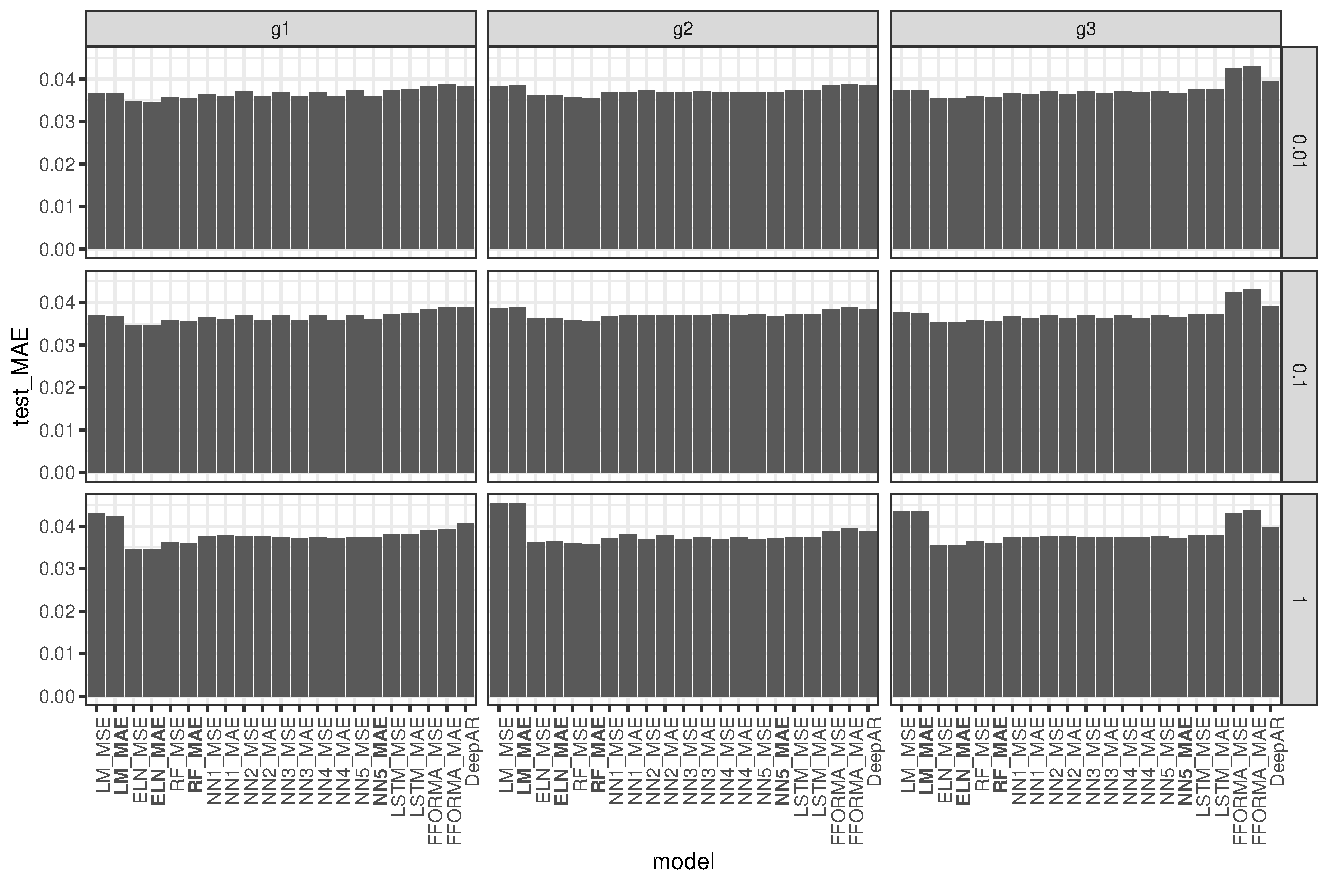
\includegraphics{simulation_test_mae.pdf}
		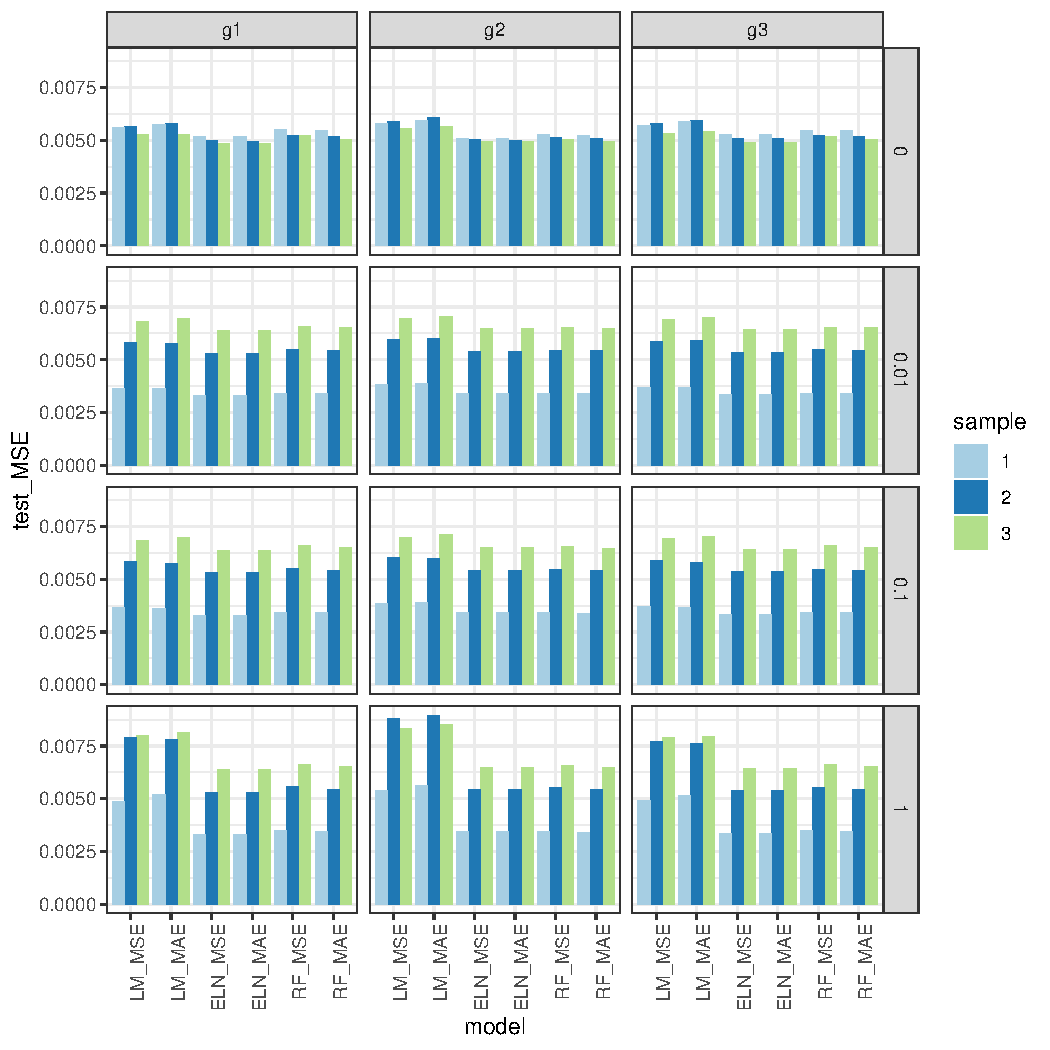
\includegraphics{simulation_test_mse.pdf}
	\end{center}
\end{table}

\begin{figure}
	\caption{Simulation Variable Importance Plots}
	\begin{center}
		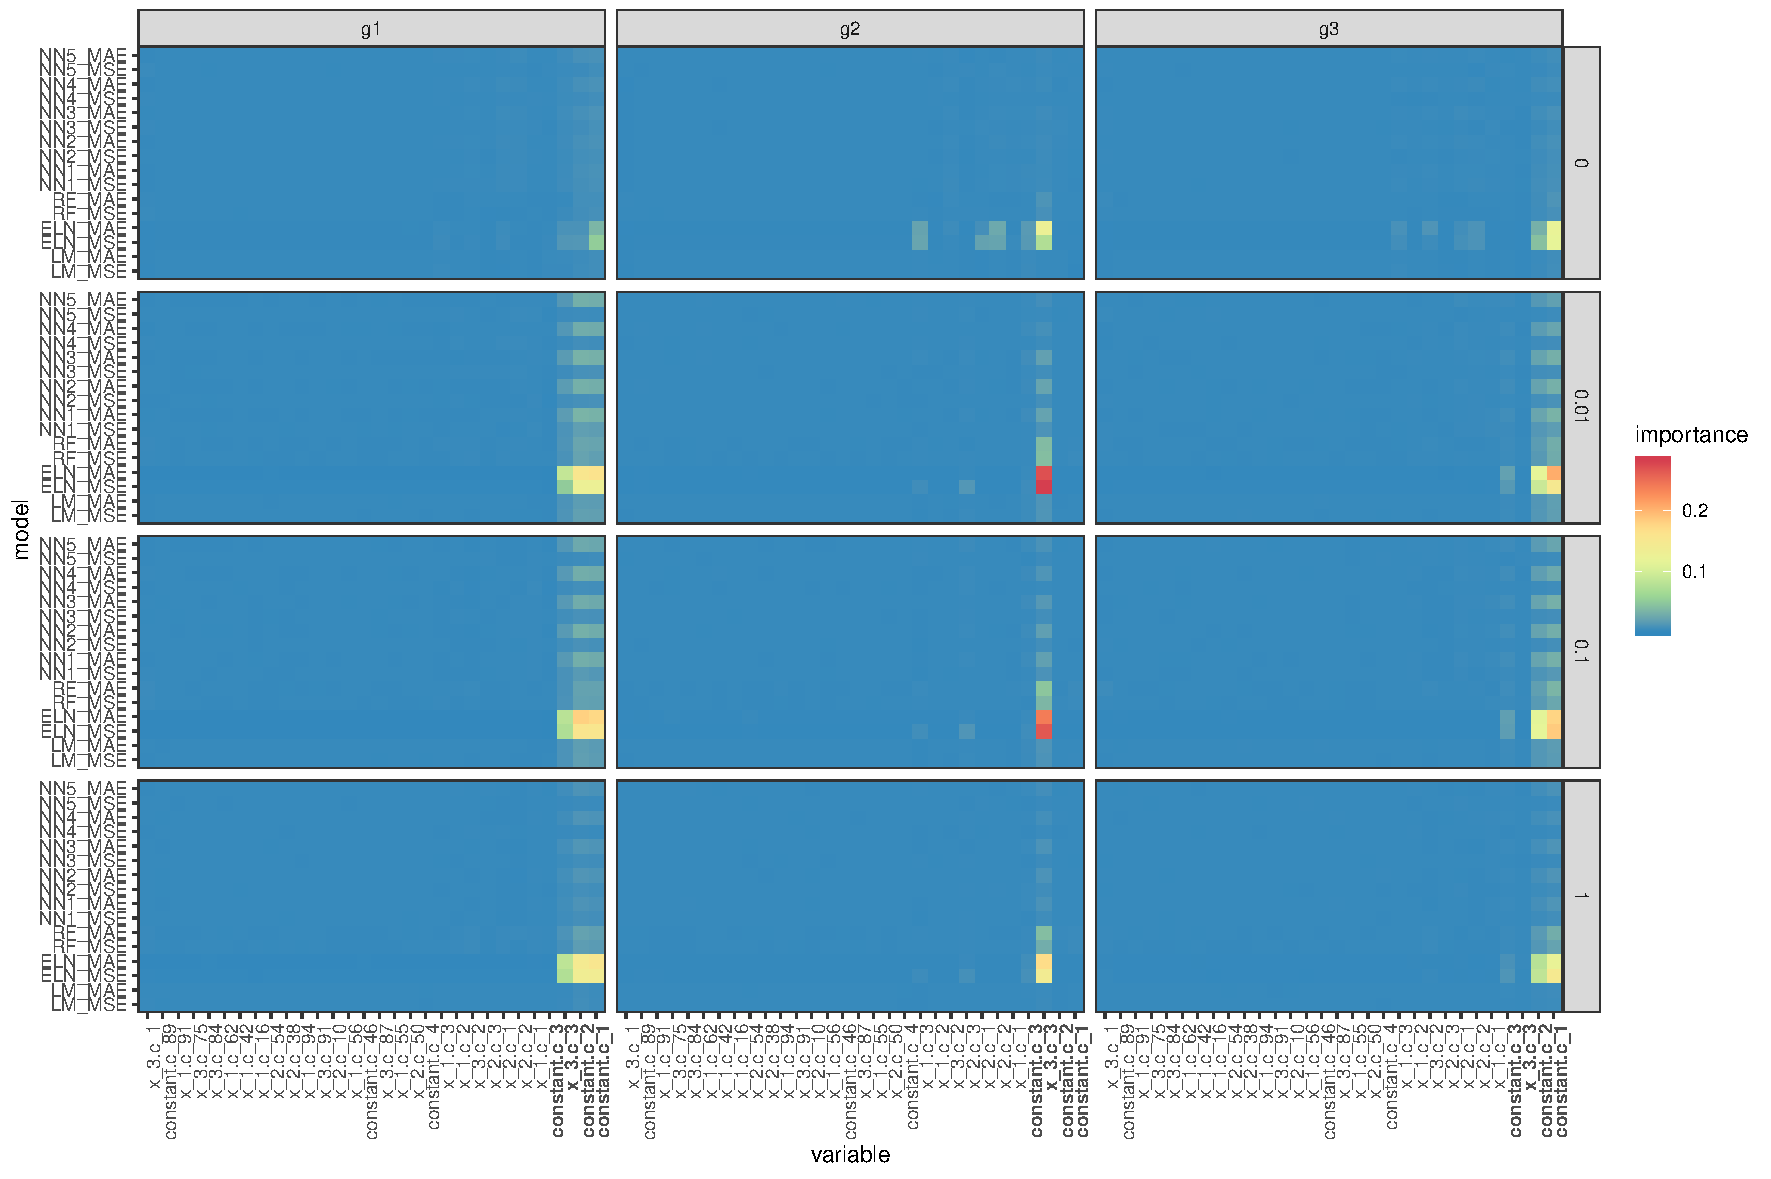
\includegraphics{simulation_ave_vi_plot.pdf}
	\end{center}
\end{figure}

%%%%%%%%%%%%%%%%%%%%%%%%%%%%%%%%%%%%%%%%%%%%%%%%%%%%%%%%%%%%%%%%%%%%%%%%%%%%%%%%%%%%%%%%%%%%%%%%%%%

\section{Empirical Study}

\subsection{Data}

% Description of original dataset
% mention how these variables are already adjusted for lags
We mimic the data procedure of \cite{gu_empirical_2018}. This means that we obtain the dataset provided by Gu on his website. This dataset sample begins in March 1957 (the start date of the S\&P 500) and ends in December 2016, totalling 60 years. It contains 94 stock level characteristics: 61 updated annually, 13 updated quarterly and 20 updated monthly, in addition to 74 industry dummies corresponding the the first two digits of the Standard Industrial Classification (SIC) codes. It is noted that this dataset contains all securities traded, including those with a CRSP share code other than 10 or 11 and thus includes instruments such as REITs and mutual funds, and those with a share price of less than \$5.

% Begin Cleaning

We detail our cleaning procedure of this dataset. To reduce the size of the dataset and increase feasibility, the dataset was filtered so that only stocks traded primarily on NASDAQ were included (using the PRIMEXCH variable from WRDS). Then, penny stocks (also referred to as microcaps in the literature) with a stock price of less than \$5 were filtered out, as is commonly done in the literature to reduce variability. Stocks without a share code of 10 or 11 (referring to equities) were filtered out, so that securities that are not equities were not included (such as REITs and trust funds). The dataset is provided in a monthly format, which means that many of the factors which are updated only quarterly or annually have very low levels of variability, which can lead to misleading results in the model fitting process. To achieve a balance between having a dataset with enough data points and variability among factors, the dataset was converted to a quarterly format. Quarterly returns were then constructed using the PRC variable according to actual returns (ie not logged differences):

\begin{equation}
	RET_t = \frac{PRC_t - PRC_{t-1}}{PRC_{t-1}}
\end{equation}

We allow all stocks which have a quarterly return to enter the dataset, even if they disappear from the dataset for certain periods, as opposed to only keeping stocks which appear continuously throughout the entire period. This was primarily done to reduce survivorship bias in the dataset, which can be very prevalent in financial data, and also allows for stocks which were unlisted and relisted again to feature in the dataset. This has the obvious drawback of introducing some bias in the dataset, as attrition in the dataset is likely to be non-random and correlated with the stocks' returns. 

The sic2 variable, corresponding to the stocks' Standard Industrial Classification (SIC) codes was also dropped. The SIC code system suffers from inconsistent logic in classifying companies, and as a system built for pre-1970s traditional industries has been slow in recognizing new and emerging industries. Indeed, WRDS explicitly cautions the use of SIC codes beyond the use of rough grouping of industries, warning that SIC codes are not strictly enforced by government agencies for accuracy, in addition to most large companies belonging to multiple SIC codes over time. Because of this latter point in particular, there can be inconsistencies on the correct SIC code for the same company depending on the data source. Dropping the sic2 variable also reduced the dimensionality of the dataset by 74 columns, significant increasing computational feasibility.

There existed a significant amount of missing data in the dataset. The dataset's columns were first examined, and any characteristics that had over 20\% of their data were removed. However, as the amount of missing data increases dramatically going further back in time, a balance between using more periods at the cost of removing more characteristics versus using less periods but keeping more characteristics was needed. 1993 Q3 was determined to be a reasonable time frame to begin the dataset, as was a noticeable increase in data availability after this time.  Missing characteristics were then imputed using their cross sectional medians for each year. 

We then follow \cite{gu_empirical_2018} and construct eight macroeconomic factors following the variable definitions in \cite{welch_comprehensive_2008}: dividend-price ratio (dp), earnings-price ratio (ep), book-to-market ratio (bm), net equity expansion (ntis), Treasury-bill rate (tbl), term spread (tms), default spread (dfy) and stock variance (svar). These factors were lagged by one period so as to be used to predict one period ahead quarterly returns. The treasury bill rate was also used from this source to proxy for the risk free rate in order to construct excess quarterly returns. 

The two sets of factors were then combined to form a baseline set of covariates, which we define throughout all methods and analysis as:

\begin{equation}
z_{i,t} = (1, x_t)' \otimes c_{i, t}
\end{equation}

where $c_{i,t}$ is a $P_c$ matrix of characteristics for each stock $i$, and $(1, x_t)'$ is a $P_x \times 1$ vector of macroeconomic predictors. $z_{i,t}$ is therefore a $P_x P_c$ vector of features for predicting individual stock returns and includes interactions between stock level characteristics and macroeconomic variables. The total number of covariates in this baseline set is $61 \times (8 + 1) = 549$\footnote{As the individual and macroeconomic factors can have similar names, individual and macroeconomic factors were prefixed with ind\_ and macro\_ respectively.}.
 
% Splitting Scheme
% Similar splitting scheme to simulation study used
% Training:Validation size ratio of 1.5, growing and moving forwards by 1 year
% To maintain feasibility, only 3 samples were conducted

The dataset was not normalized for all methods, as only penalized regression and neural networks are sensitive to normalization. For these two methods, the dataset was normalized such that each predictor column had 0 mean and 1 variance.

The final dataset spanned from 1993 Q3 to 2016 Q4 with 202066 individual observations.

We mimic the procedure used in the simulation study. This means that the dataset was split such that the training and validation sets were split such that the training set was approximately 1.5 times the length of the validation set, in order to predict a test set that is one year in length.

\begin{figure}
	\begin{center}
		\begin{tabular}{|c|p{0.50cm}p{0.50cm}p{0.50cm}p{0.50cm}p{0.50cm}p{0.50cm}p{0.50cm}p{0.50cm}p{0.50cm}p{0.50cm}p{0.50cm}p{0.50cm}p{0.50cm}p{0.50cm}p{0.50cm}p{0.50cm}|}
			\hline
			Set No. &&&&&&&&&&&&&&&& \\
			\hline
			%%%%%%%%
			3 & \cellcolor{cyan} & \cellcolor{cyan} & \cellcolor{cyan} & \cellcolor{cyan} & \cellcolor{cyan} & \cellcolor{cyan} & \cellcolor{cyan} & \cellcolor{cyan} &
			\cellcolor{pink} & \cellcolor{pink} & \cellcolor{pink} & \cellcolor{pink} & \cellcolor{pink} & \cellcolor{pink} & \cellcolor{pink} & \cellcolor{olive} \\
			%%%%%%%%
			2 & \cellcolor{cyan} & \cellcolor{cyan} & \cellcolor{cyan} & \cellcolor{cyan} & \cellcolor{cyan} & \cellcolor{cyan} & \cellcolor{cyan} &
			\cellcolor{pink} & \cellcolor{pink} & \cellcolor{pink} & \cellcolor{pink} & \cellcolor{pink} & \cellcolor{pink} & \cellcolor{pink} & 	
			\cellcolor{olive} & NA \\
			%%%%%%%%
			1 & \cellcolor{cyan} & \cellcolor{cyan} & \cellcolor{cyan} & \cellcolor{cyan} & \cellcolor{cyan} & \cellcolor{cyan} &
			\cellcolor{pink} & \cellcolor{pink} & \cellcolor{pink} & \cellcolor{pink} & \cellcolor{pink} & \cellcolor{pink} & \cellcolor{pink} & \cellcolor{olive} & NA & NA \\
			\hline
			Time & 1993Q3 & 1993Q4 & 1994 & 1995 & 1996 & ... & 2006 & 2007 & 2008 & ... & 2011 & 2012 & 2013 & 2014 & 2015 & 2016 \\
			\hline
		\end{tabular}
		\medskip
		\begin{tabular}{|c|p{0.60cm}|}
			\hline
			Training & \cellcolor{cyan} \\
			\hline
			Validation & \cellcolor{pink} \\
			\hline
			Test & \cellcolor{olive} \\
			\hline
		\end{tabular}
	\end{center}
	\caption{Empirical Data Sample Splitting Procedure}
	\label{emp_sample_split_diag}
\end{figure}

\newpage

\subsection{Empirical Data Results}

\subsubsection{Prediction Accuracy}

In general, results from the simulation study were reproduced in the empirical study. We similarly see that the penalized linear models generally performing the best, with the random forest models offering slightly worse performance, occasionally outperforming penalized linear models. Models fitted with respect to median quantile loss were similarly observed to typically offer improvements across all machine learning models across all loss metrics.

In the empirical data setting, the underlying data generating process of returns is unknown so the ability of the different models at picking out the correct covariates cannot be evaluated. However, we can see that the penalized linear models and random forests (the models with the highest out of sample prediction performance) decide on a similar subset of factors which are determined to be important. In particular, we find that the 1 month momentum and 6 month momentum factors to be the most important factors by far, and this is consistent across all training samples. The conservative sparsity of the penalized linear models seen in the simulated setting is not repeated here; almost all factors are assigned to have small importance. The random forests again seem to struggle with discerning the importance of correlated factors apart: many of the important factors identified are highly correlated with momentum, such as change in momentum, dollar trading volume and return volatility.

The linear models had the worst performance of all the models considered. Interestingly, we find that the linear models assign the controversial dividend price ratio macroeconomic factor as highly important. Their variable importance for individual factors across different training samples is highly non-robust, with the important variables almost completely changing year to year.

The neural networks similarly had non-robust results. There is weak evidence to suggest that more complex neural networks with more layers give better performance. The neural networks were also the only models to assign high variable importance to the individual market value factor, a result that is somewhat consistent across all neural networks considered. 

All models considered typically preferred sparse parameterizations. That is, most if not all of the individual factors had little to no importance across all models. 

When looking at the macroeconomic factors (see Figure \ref{empirical_macro_facet}), there is less consistency on the variable importance between models. Penalized linear models tend to identify the average book to market ratio and the default spread as the most important macroeconomic factors, a result weakly consistent with those of the random forests. The linear models consistently identified the controversial dividend-price ratio as important, a result that was somewhat consistent with the neural networks. Some of the neural networks also occasionally identified the earnings price ratio as important.

\begin{figure}
	\begin{center}
		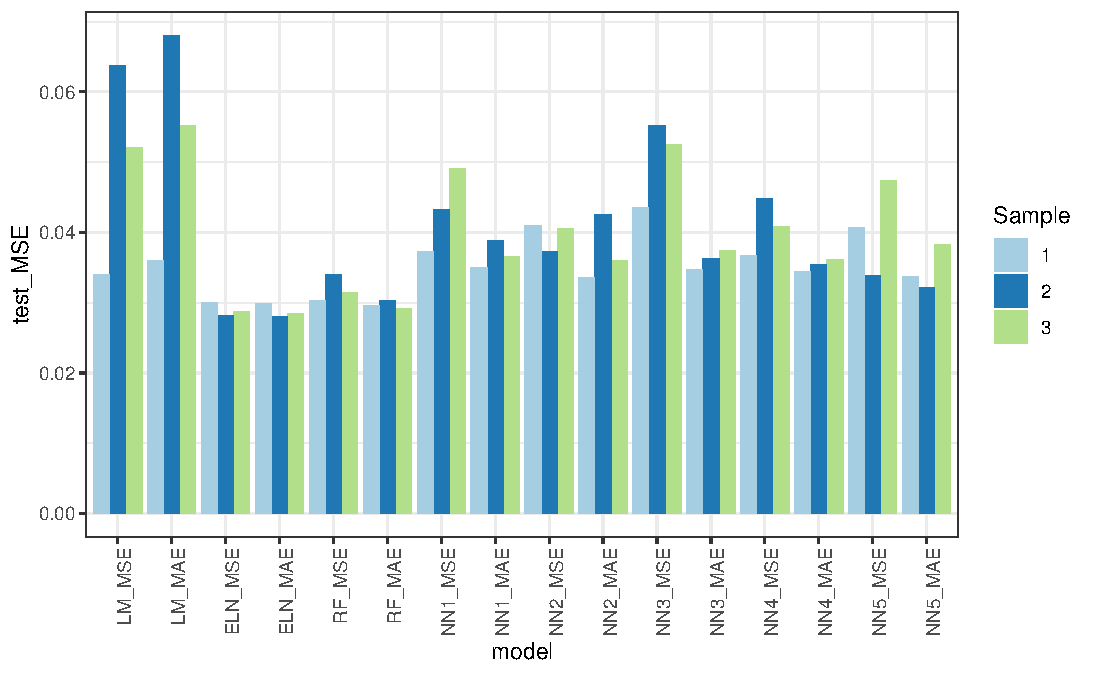
\includegraphics{empirical_test_mse}
	\end{center}
	\caption{Empirical Test MSE Averaged Across All Samples}
\end{figure}

\begin{figure}
	\begin{center}
		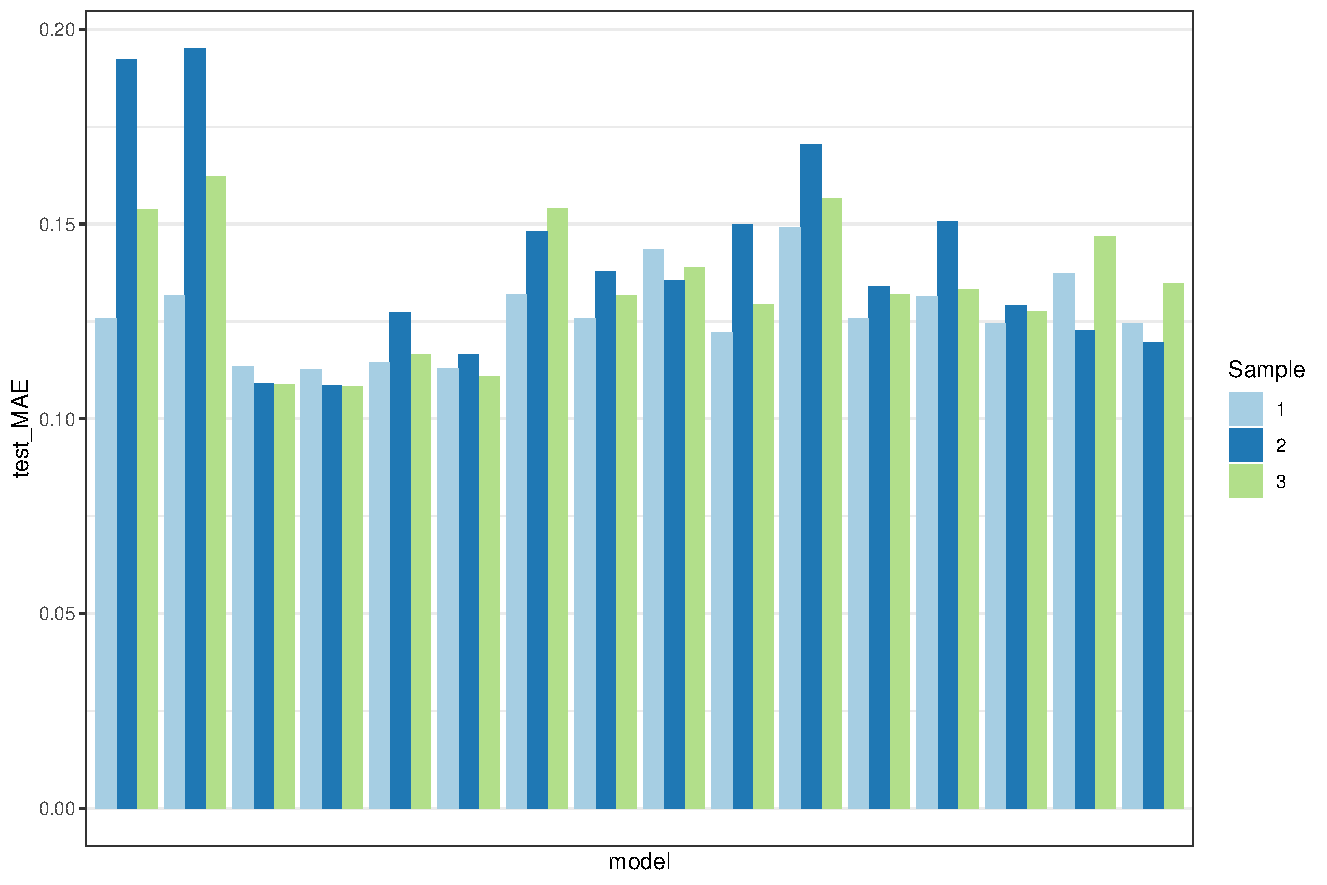
\includegraphics{empirical_test_mae}
	\end{center}
	\caption{Empirical Test MAE Averaged Across All Samples}
\end{figure}

\newpage

\begin{figure}
	\begin{center}
	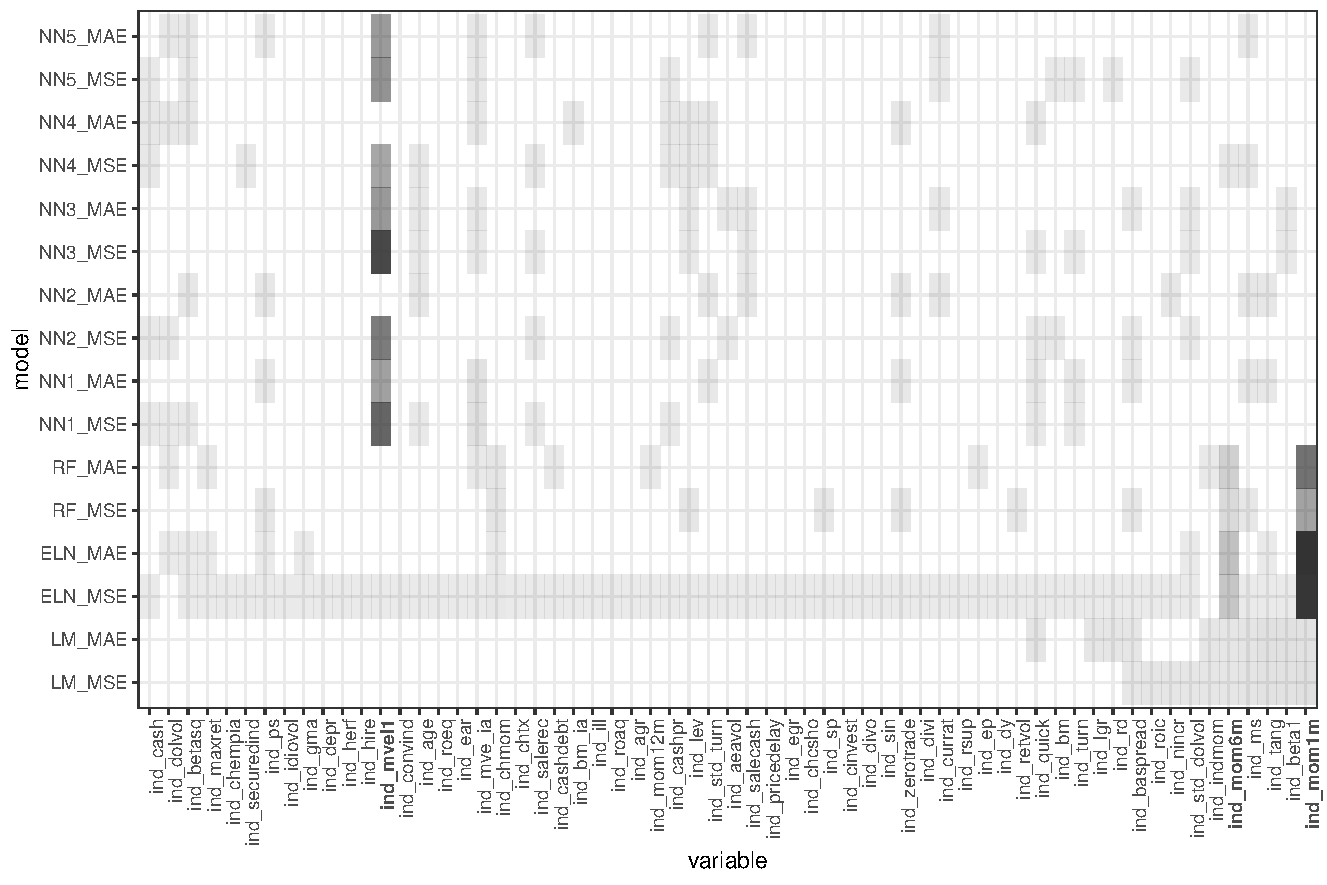
\includegraphics{empirical_sample_all_vi_ind.pdf}
	\end{center}
	\caption{Empirical Data Individual Factor Variable Importance Averaged Across All Samples}
\end{figure}

\begin{figure}
	\begin{center}
	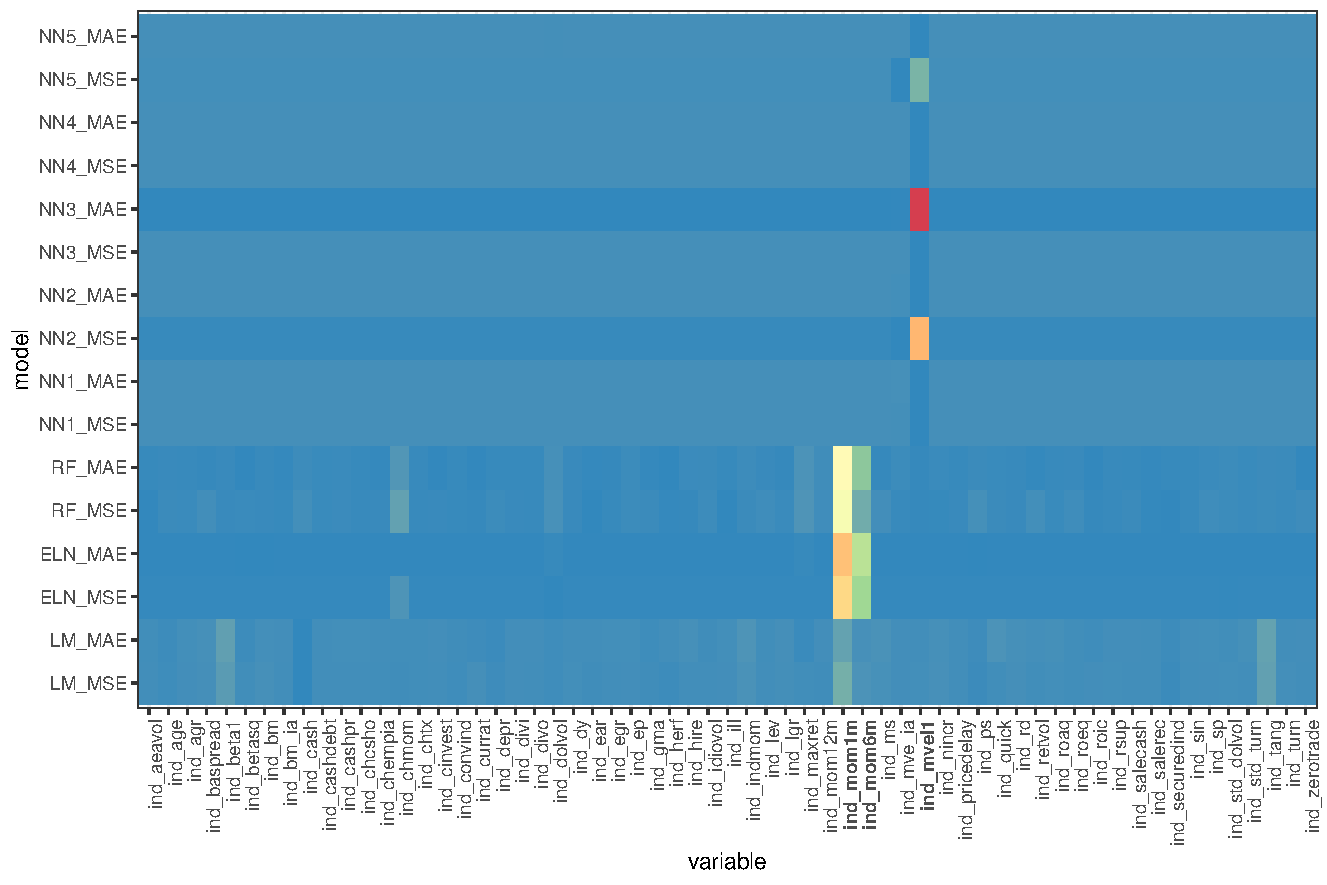
\includegraphics{empirical_sample_1_vi_ind.pdf}
	\end{center}
	\caption{Empirical Data Individual Factor Variable Importance for Sample 1}
\end{figure}

\begin{figure}
	\begin{center}
	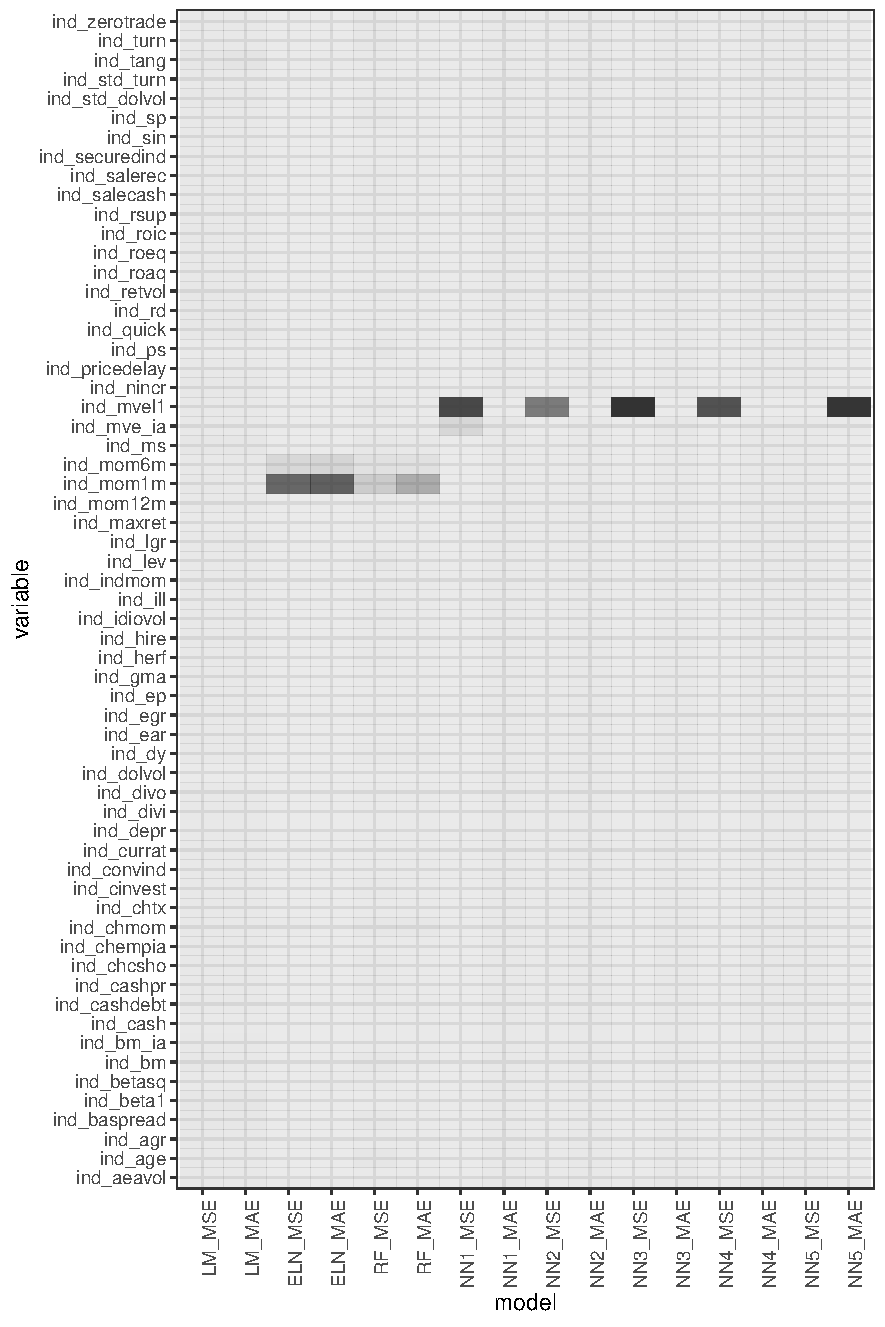
\includegraphics{empirical_sample_2_vi_ind.pdf}
	\end{center}
	\caption{Empirical Data Individual Factor Variable Importance for Sample 2}
\end{figure}

\begin{figure}
	\begin{center}
	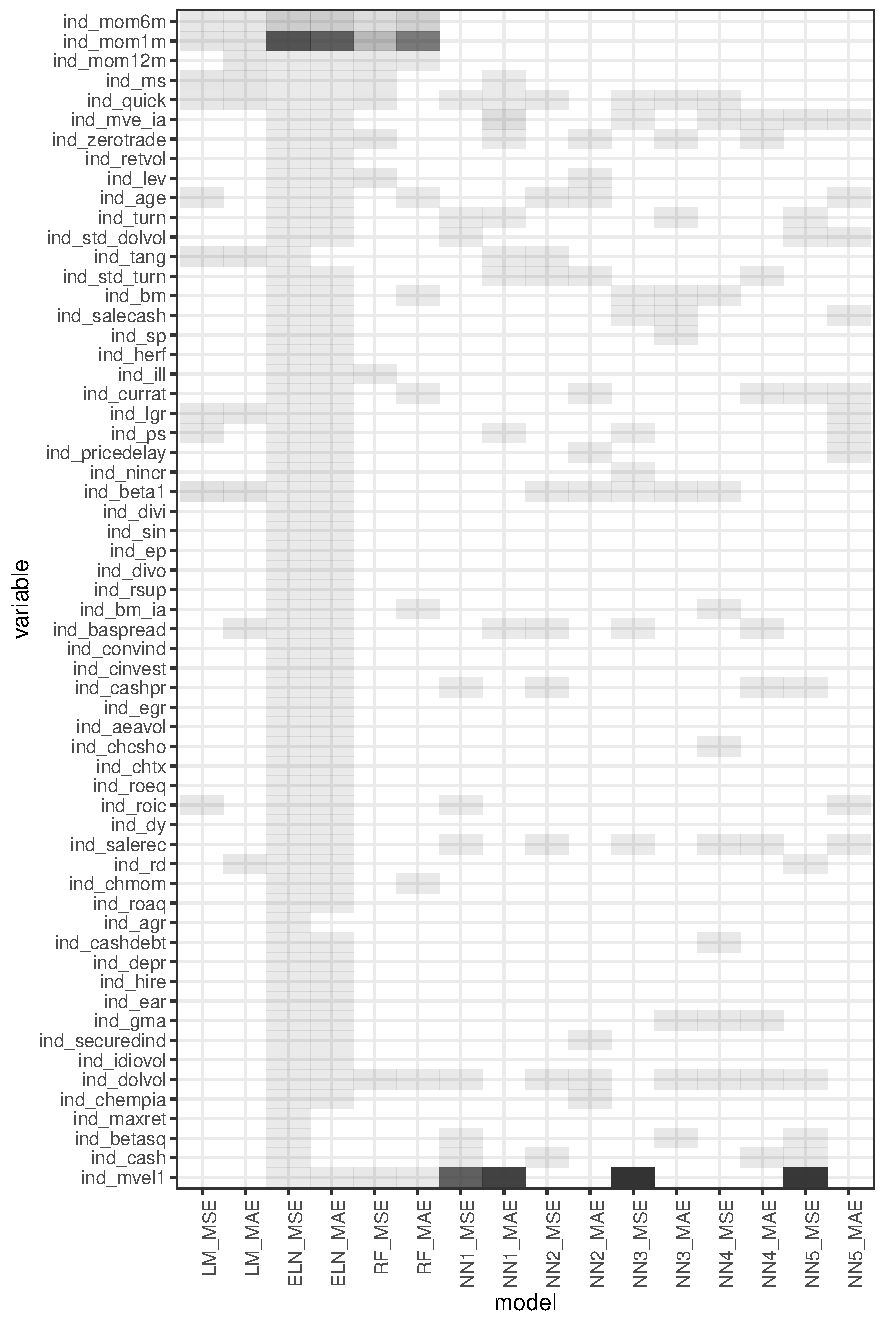
\includegraphics{empirical_sample_3_vi_ind.pdf}
	\end{center}
	\caption{Empirical Data Individual Factor Variable Importance for Sample 3}
\end{figure}

\begin{landscape}
\begin{figure}
	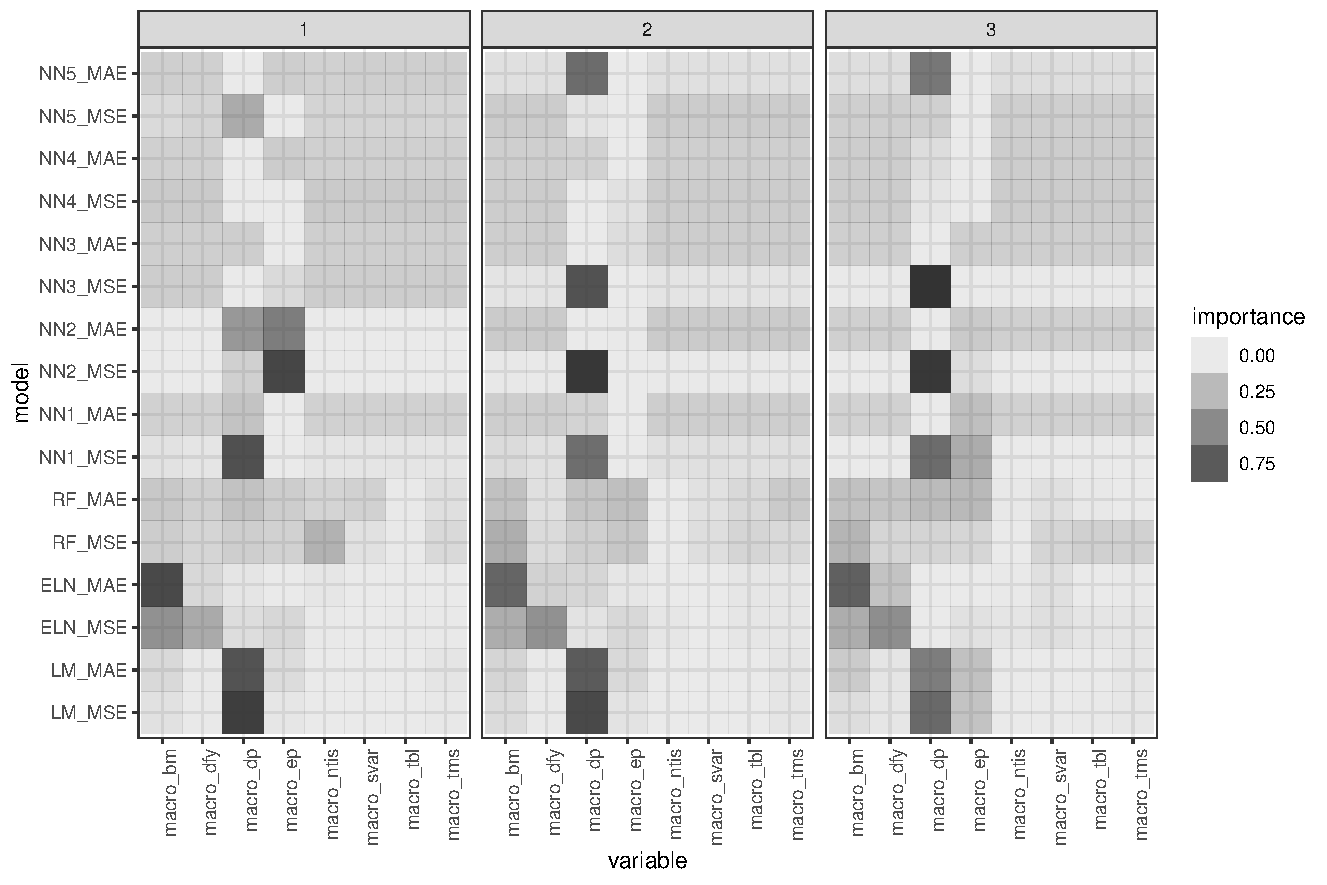
\includegraphics{empirical_sample_all_vi_macro_facet.pdf}
	\caption{Empirical Data Macroeconomic Factor variable Importance Averaged Across All Samples, faceted by training sample}
	\label{empirical_macro_facet}
\end{figure}
\end{landscape}

\section{Conclusion}

Our findings demonstrate that within the contexts considered, the field of machine learning offers tools to improve stock prediction and identification of true underlying regressors. Penalized linear models and to a lesser extent, random forests are the best performing methods.

Importantly, we find that the feed-forward neural network architectures considered fail in the context of stock return prediction, at both prediction performance and variable importance analysis. This is a result consistent across a variety of simulated datasets, as well as empirical data. We also find weak evidence that deeper neural networks with more hidden layers perform better, though this result, like the performance of neural networks in general, is non-robust.

Lastly, we find that the top performing models - the penalized linear models and random forests, tend to agree and correctly identify the correct causal regressors in simulated contexts, as well as agree on the same subset of factors which are important in empirical contexts. We find that the of all the most considered, the penalized linear models are the most consistent at identifying true causal regressors through the simulation study. We find that in the empirical setting, among the individual the individual 1 and 6 month momentum factors are the most powerful predictors of stock returns, according to the penalized linear models and random forests. 

Across all models except for linear models, we find that minimizing quantile loss yields better prediction performance.

The overall findings of this paper differ from the sparse literature on similar topics. However, the performance of the penalized linear models with respect to both out of sample prediction performance and variable importance analysis is promising, and our findings show that machine learning provides some tools which may aid in the problems of stock return prediction and risk factor selection in the financial world. 

\newpage

\section{Appendix}

\subsection{Data}

%% Individual Factor Table

\begin{landscape}
	\footnotetext{The factor was included in the original dataset provided by \cite{gu_empirical_2018}, but was not used due to missing data issues}
	\begin{center}
		\label{ind_factors}
		\begin{longtable}{lllllll}
			\caption{Individual Factors} \\ \hline
			No. & Acronym & Firm Characteristic & Author(s) & Data Source & Frequency \\ \hline
			1 & ind\_absacc\footnotemark[\value{footnote}] & Absolute Accruals & 
				\cite{bandyopadhyay_accrual_2010} & Compustat & Annual \\
			2 & ind\_acc\footnotemark[\value{footnote}] & Working capital accruals & 
				\cite{sloan_stock_1996} & Compustat & Annual \\
			3 & ind\_aeavol & Abnormal earnings announcement volume & 
				\cite{lerman_high-volume_2008} & Compustat & Quarterly \\
			4 & ind\_age & \# years since first Compustat coverage & 
				\cite{jiang_information_2005} & Compustat & Annual \\
			5 & ind\_agr & Asset growth & 
				\cite{cooper_asset_2008} & Compustat & Annual \\
			6 & ind\_baspread & Bid-ask spread & 
				\cite{amihud_effects_1989} & Compustat & Monthly \\
			7 & ind\_beta & Beta & 
				\cite{fama_risk_1973} & Compustat & Monthly \\
			8 & ind\_betasq & Beta squared & 
				\cite{fama_risk_1973} & Compustat & Monthly \\
			9 & ind\_bm & Book-to-market & 
				\cite{rosenberg_persuasive_1985} & Compustat & Annual \\
			10 & ind\_bm\_ia & Industry-adjusted book to market & 
				\cite{asness_predicting_2000} & Compustat & Quarterly \\
			%%%%%%%%%%%%%%%%%%%%%%%%%%%%%%%%%%%%%%%%%%%%%%%%%%%%%%%%%%%%%%%%%%%%%%%%%%%%%%%
			11 & ind\_cash & Cash holdings & 
				\cite{palazzo_cash_2012} & Compustat & Annual \\
			12 & ind\_cashdebt & Cashflow to debt & 
				\cite{ou_financial_1989} & Compustat & Annual \\
			13 & ind\_cashpr & Cash productivity & 
				\cite{chandrashekar_productivity_2009} & Compustat & Annual \\
			14 & ind\_cfp\footnotemark[\value{footnote}] & Cashflow to price ratio & 
				\cite{desai_value-glamour_2004} & Compustat & Annual \\
			15 & ind\_cfp\_ia\footnotemark[\value{footnote}] & Industry-adjusted cashfow to price ratio & 
				\cite{asness_predicting_2000} & Compustat & Annual \\
			16 & ind\_chatoia\footnotemark[\value{footnote}] & Industry-adjusted change in asset turnover & 
				\cite{soliman_use_2008} & Compustat & Annual \\
			17 & ind\_chcsho & Change in shares outstanding & 
				\cite{pontiff_share_2008} & Compustat & Annual \\
			18 & ind\_chempia & Industry-adjusted change in employee & 
				\cite{asness_predicting_2000} & Compustat & Annual \\
			19 & ind\_chinv\footnotemark[\value{footnote}] & Change in inventory & 
				\cite{thomas_inventory_2002} & Compustat & Annual \\
			%%%%%%%%%%%%%%%%%%%%%%%%%%%%%%%%%%%%%%%%%%%%%%%%%%%%%%%%%%%%%%%%%%%%%%%%%%%%%%%
			20 & ind\_chmom & Change in 6-month momentum & 
				\cite{gettleman_acceleration_2006} & Compustat & Monthly \\
			21 & ind\_chpmia\footnotemark[\value{footnote}] & Industry-adjusted change in profit margin & 
				\cite{soliman_use_2008} & Compustat & Annual \\
			22 & ind\_chtx & Change in tax expense & 
				\cite{thomas_tax_2011} & Compustat & Quarterly \\
			23 & ind\_cinvest & Corporate investment & 
				\cite{titman_capital_2004} & Compustat & Quarterly \\
			24 & ind\_convind & Convertible debt indicator & 
				\cite{valta_strategic_2016} & Compustat & Annual \\
			25 & ind\_currat & Current ratio & 
				\cite{ou_financial_1989} & Compustat & Annual \\
			26 & ind\_depr & Depreciation / PP\&E & 
				\cite{holthausen_prediction_1992} & Compustat & Annual \\
			27 & ind\_divi & Dividend initiation & 
				\cite{michaely_price_1995} & Compustat & Annual \\
			28 & ind\_divo & Dividend omission & 
				\cite{michaely_price_1995} & Compustat & Annual \\
			29 & ind\_dolvol & Dollar trading volume & 
				\cite{chordia_trading_2001} & Compustat & Monthly \\
			%%%%%%%%%%%%%%%%%%%%%%%%%%%%%%%%%%%%%%%%%%%%%%%%%%%%%%%%%%%%%%%%%%%%%%%%%%%%%%%
			30 & ind\_dy & Dividend to price & 
				\cite{litzenberger_effects_1982} & Compustat & Annual \\
			31 & ind\_ear & Earnings announcement return & 
				\cite{brandt_earnings_2008} & Compustat & Quarterly \\
			32 & ind\_egr & Growth in common shareholder eq & 
				\cite{richardson_accrual_2005} & Compustat & Annual \\
			33 & ind\_ep & Earnings to price & 
				\cite{basu_investment_1977} & Compustat & Annual \\
			34 & ind\_gma & Gross profitability & 
				\cite{novy-marx_other_2013} & Compustat & Annual \\
			35 & ind\_grCAPX\footnotemark[\value{footnote}] & Growth in capital expenditures & 
				\cite{anderson_empirical_2006} & Compustat & Annual \\
			36 & ind\_grltnoa\footnotemark[\value{footnote}] & Growth in long term net operating assets & 
				\cite{fairfield_accrued_2003} & Compustat & Annual \\
			37 & ind\_herf & Industry sales concentration & 
				\cite{hou_industry_2006} & Compustat & Annual \\
			38 & ind\_hire & Employee growth rate & 
				\cite{belo_labor_2014} & Compustat & Annual \\
			39 & ind\_idiovol & Idiosyncratic return volatility & 
				\cite{ali_arbitrage_2003} & Compustat & Monthly \\
			%%%%%%%%%%%%%%%%%%%%%%%%%%%%%%%%%%%%%%%%%%%%%%%%%%%%%%%%%%%%%%%%%%%%%%%%%%%%%%%
			40 & ind\_ill & Illiquidity & 
				\cite{amihud_illiquidity_2002} & Compustat & Monthly \\
			41 & ind\_indmom & Industry momentum & 
				\cite{moskowitz_industries_1999} & Compustat & Monthly \\
			42 & ind\_invest\footnotemark[\value{footnote}] & Capital expenditures and inventory & 
				\cite{chen_better_2010} & Compustat & Annual \\
			43 & ind\_lev & Leverage & 
				\cite{bhandari_debt/equity_1988} & Compustat & Annual \\
			44 & ind\_lgr & Growth in long-term debt & 
				\cite{richardson_accrual_2005} & Compustat & Annual \\
			45 & ind\_maxret & Maximum daily return & 
				\cite{bali_maxing_2011} & Compustat & Monthly \\
			46 & ind\_mom12m & 12-month momentum & 
				\cite{jegadeesh_evidence_1990} & Compustat & Monthly \\
			47 & ind\_mom1 & 1-month momentum & 
				\cite{jegadeesh_returns_1993} & Compustat & Monthly \\
			48 & ind\_mom36m\footnotemark[\value{footnote}] & 36-month momentum & 
				\cite{jegadeesh_returns_1993} & Compustat & Monthly \\
			49 & ind\_mom6m & 6-month momentum & 
				\cite{jegadeesh_returns_1993} & Compustat & Monthly \\
			%%%%%%%%%%%%%%%%%%%%%%%%%%%%%%%%%%%%%%%%%%%%%%%%%%%%%%%%%%%%%%%%%%%%%%%%%%%%%%%
			50 & ind\_ms & Financial statement score & 
				\cite{mohanram_separating_2005} & Compustat & Quarterly \\
			51 & ind\_mvel1 & Size & 
				\cite{banz_relationship_1981} & Compustat & Monthly \\
			52 & ind\_mve\_ia & Industry-adjusted size & 
				\cite{asness_predicting_2000} & Compustat & Annual \\
			53 & ind\_nincr & Number of earnings increases & 
				\cite{barth_market_1999} & Compustat & Quarterly \\
			54 & ind\_operprof\footnotemark[\value{footnote}] & Operating profitability & 
				\cite{fama_five-factor_2015} & Compustat & Annual \\
			55 & ind\_orgcap\footnotemark[\value{footnote}] & Organizational capital & 
				\cite{eisfeldt_organization_2013} & Compustat & Annual \\
			56 & ind\_pchcapx\_ia\footnotemark[\value{footnote}] & Industry adjusted \% change in capital expenditures & 
				\cite{abarbanell_abnormal_1998} & Compustat & Annual \\
			57 & ind\_pchcurrat\footnotemark[\value{footnote}] & \% change in current ratio & 
				\cite{ou_financial_1989} & Compustat & Annual \\
			58 & ind\_pchdepr\footnotemark[\value{footnote}] & \% change in depreciation & 
				\cite{holthausen_prediction_1992} & Compustat & Annual \\
			59 & ind\_pchgm\_pchsale\footnotemark[\value{footnote}] & \% change in gross margin - \% change in sales & 
				\cite{abarbanell_abnormal_1998} & Compustat & Annual \\
			%%%%%%%%%%%%%%%%%%%%%%%%%%%%%%%%%%%%%%%%%%%%%%%%%%%%%%%%%%%%%%%%%%%%%%%%%%%%%%%
			60 & ind\_pchquick\footnotemark[\value{footnote}] & \% change in quick ratio & 
				\cite{ou_financial_1989} & Compustat & Annual \\
			61 & ind\_pchsale\_pchinvt\footnotemark[\value{footnote}] & \% change in sales - \% change in inventory & 
				\cite{abarbanell_abnormal_1998} & Compustat & Annual \\
			62 & ind\_pchsale\_pchrect\footnotemark[\value{footnote}] & \% change in sales - \% change in A/R & 
				\cite{abarbanell_abnormal_1998} & Compustat & Annual \\
			63 & ind\_pchsale\_pchxsga\footnotemark[\value{footnote}] & \% change in sales - \% change in SG & 
				\cite{abarbanell_abnormal_1998} & Compustat & Annual \\
			64 & ind\_pchsaleinv\footnotemark[\value{footnote}] & \% change sales-to-inventory & 
				\cite{ou_financial_1989} & Compustat & Annual \\
			65 & ind\_pctacc\footnotemark[\value{footnote}] & Percent accruals & 
				\cite{hafzalla_percent_2011} & Compustat & Annual \\
			66 & ind\_pricedelay & Price delay & 
				\cite{hou_market_2005} & Compustat & Monthly \\
			67 & ind\_ps & Financial statements score & 
				\cite{piotroski_value_2000} & Compustat & Annual \\
			68 & ind\_quick & Quick ratio & 
				\cite{ou_financial_1989} & Compustat & Annual \\
			69 & ind\_rd & R\&D increase & 
				\cite{eberhart_examination_2004} & Compustat & Annual \\
			%%%%%%%%%%%%%%%%%%%%%%%%%%%%%%%%%%%%%%%%%%%%%%%%%%%%%%%%%%%%%%%%%%%%%%%%%%%%%%%
			70 & ind\_rd\_mve\footnotemark[\value{footnote}] & R\&D to market capitalization & 
				\cite{guo_explaining_2006} & Compustat & Annual \\
			71 & ind\_rd\_sale\footnotemark[\value{footnote}] & R\&D to sales & 
				\cite{guo_explaining_2006} & Compustat & Annual \\
			72 & ind\_realestate\footnotemark[\value{footnote}] & Real estate holdings & 
				\cite{tuzel_corporate_2010} & Compustat & Annual \\
			73 & ind\_retvol & Return volatility & 
				\cite{ang_cross-section_2006} & Compustat & Monthly \\
			74 & ind\_roaq & Return on assets & 
				\cite{balakrishnan_post_2010} & Compustat & Quarterly \\
			75 & ind\_roavol\footnotemark[\value{footnote}] & Earnings volatility & 
				\cite{francis_costs_2004} & Compustat & Quarterly \\
			76 & ind\_roeq & Return on equity & 
				\cite{hou_digesting_2015} & Compustat & Quarterly \\
			77 & ind\_roic & Return on invested capital & 
				\cite{brown_productivity_2007} & Compustat & Annual \\
			78 & ind\_rsup & Revenue surprise & 
				\cite{kama_market_2009} & Compustat & Quarterly \\
			79 & ind\_salecash & Sales to cash & 
				\cite{ou_financial_1989} & Compustat & Annual \\
			%%%%%%%%%%%%%%%%%%%%%%%%%%%%%%%%%%%%%%%%%%%%%%%%%%%%%%%%%%%%%%%%%%%%%%%%%%%%%%%
			80 & ind\_saleinv\footnotemark[\value{footnote}] & Sales to inventory & 
				\cite{ou_financial_1989} & Compustat & Annual \\
			81 & ind\_salerec & Sales to receivables & 
				\cite{ou_financial_1989} & Compustat & Annual \\
			82 & ind\_secured\footnotemark[\value{footnote}] & Secured debt & 
				\cite{valta_strategic_2016} & Compustat & Annual \\
			83 & ind\_securedind & Secured debt indicator & 
				\cite{valta_strategic_2016} & Compustat & Annual \\
			84 & ind\_sgr\footnotemark[\value{footnote}] & Sales growth & 
				\cite{barbee_jr_salesprice_1996} & Compustat & Annual \\
			85 & ind\_sin & Sin stocks & 
				\cite{hong_price_2009} & Compustat & Annual \\
			86 & ind\_sp & Sales to price & 
				\cite{barbee_jr_salesprice_1996} & Compustat & Annual \\
			87 & ind\_std\_dolvol & Volatility of liquidity (dollar trading volume) & 
				\cite{chordia_trading_2001} & Compustat & Annual \\
			88 & ind\_std\_turn & Volatility of liquidity (share turnover) & 
				\cite{chordia_trading_2001} & Compustat & Monthly \\
			89 & ind\_stdacc\footnotemark[\value{footnote}] & Accrual volatility & 
				\cite{bandyopadhyay_accrual_2010} & Compustat & Monthly \\
			%%%%%%%%%%%%%%%%%%%%%%%%%%%%%%%%%%%%%%%%%%%%%%%%%%%%%%%%%%%%%%%%%%%%%%%%%%%%%%%
			90 & ind\_stdcf\footnotemark[\value{footnote}] & Cashflow volatility & 
				\cite{huang_cross_2009} & Compustat & Quarterly \\
			91 & ind\_tang & Debt capacity/rm tangibility & 
				\cite{almeida_financial_2007} & Compustat & Quarterly \\
			92 & ind\_tb\footnotemark[\value{footnote}] & Tax income to book income & 
				\cite{lev_market-based_1982} & Compustat & Annual \\
			93 & ind\_turn & Share turnover & 
				\cite{datar_liquidity_1998} & Compustat & Monthly \\
			94 & ind\_zerotrade & Zero trading days & 
				\cite{liu_liquidity-augmented_2006} & Compustat & Monthly \\ \hline	
		\end{longtable}
	\end{center}
\end{landscape}

\newpage

%% Macroeconomic Factor Table

\begin{table}
	\caption{Macroeconomic Factors}
	\begin{center}
	\begin{tabular}{lccc} \hline
		No. & Acronym & Macroeconomic Factor \\ \hline
		1 & macro\_dp & Dividend Price Ratio \\
		2 & macro\_ep & Earnings Price Ratio \\
		3 & macro\_bm & Book to Market Ratio \\
		4 & macro\_ntis & Net Equity Expansion \\
		5 & macro\_tbl & Treasury Bill Rate \\
		6 & macro\_tms & Term Spread \\
		7 & macro\_dfy & Default Spread \\
		8 & macro\_svar & Stock Variance \\ \hline
	\end{tabular}
	\end{center}
\end{table}

\newpage

\subsection{Additional Results}

\subsubsection{Simulation Study}

\begin{figure}
	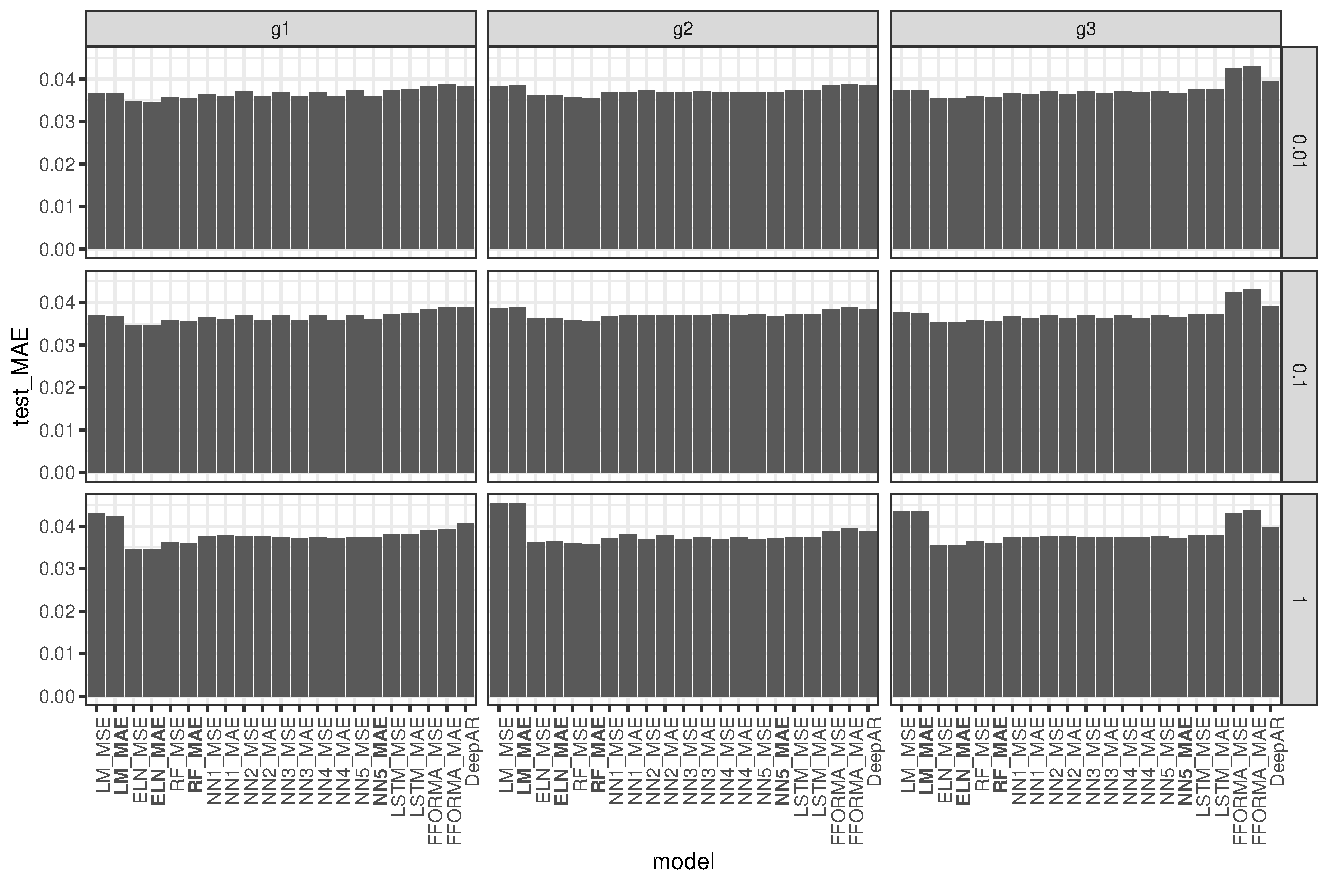
\includegraphics{simulation_test_mae.pdf}
	\caption{Simulation Test MAE}
\end{figure}

\begin{figure}
	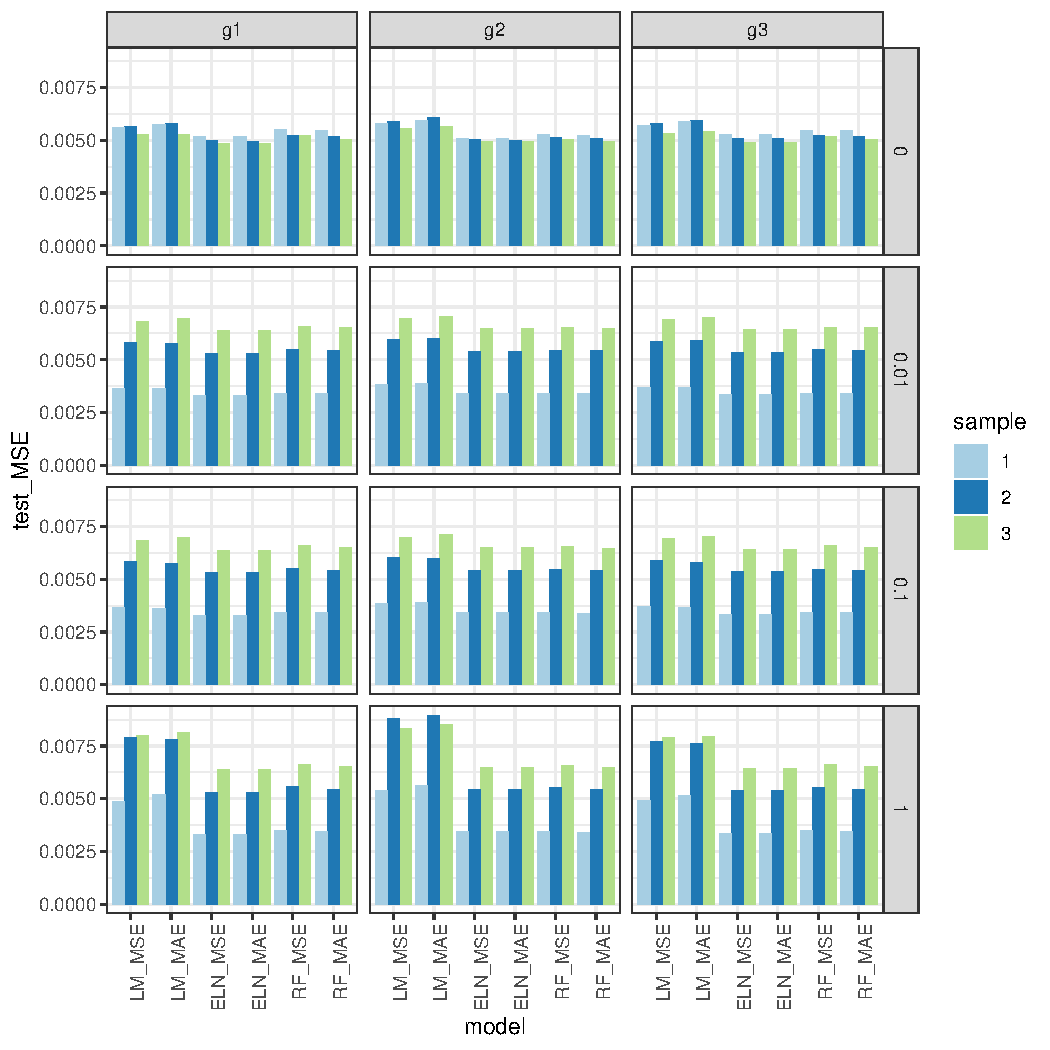
\includegraphics{simulation_test_mse.pdf}
	\caption{Simulation Test MSE}
\end{figure}

\begin{figure}
	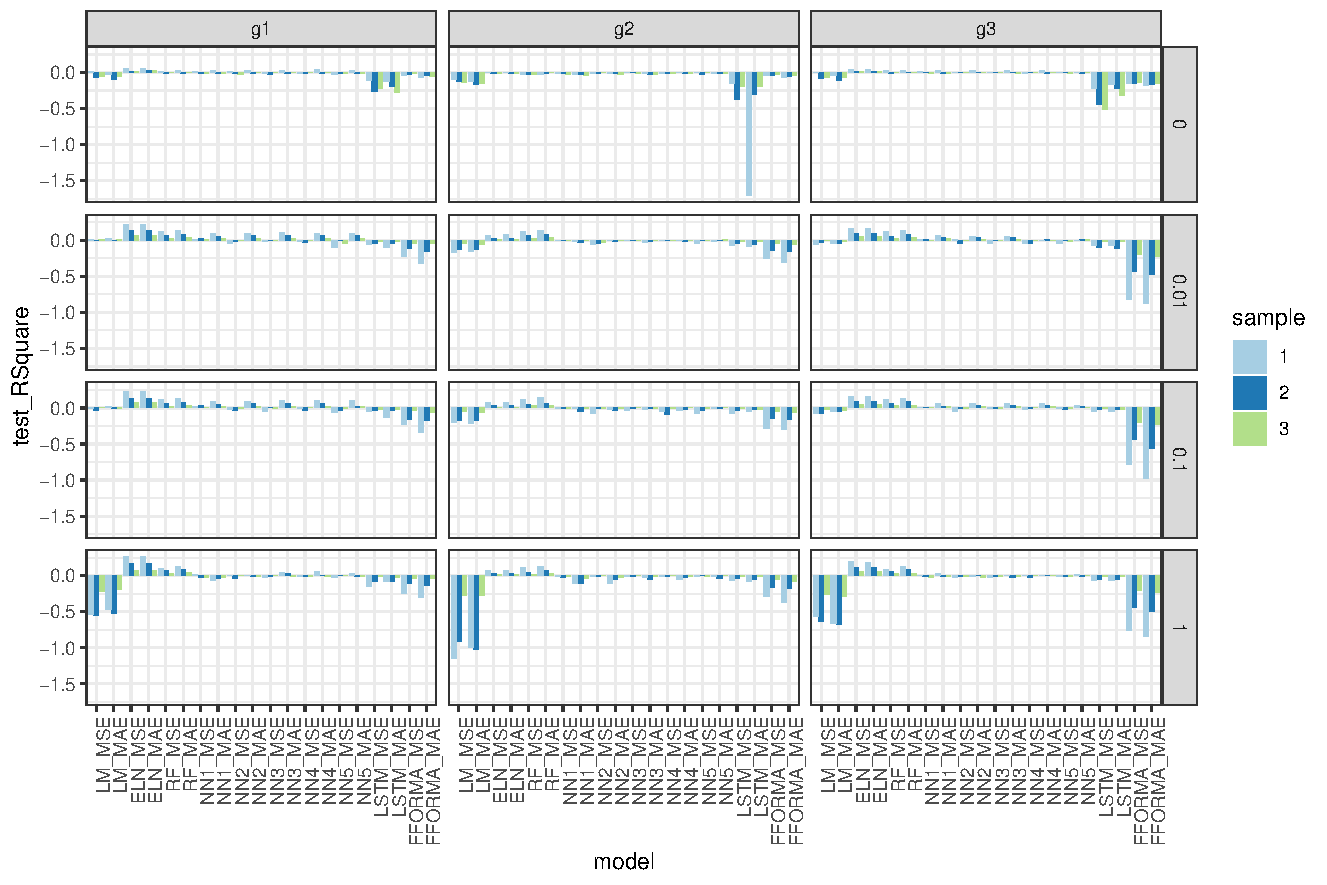
\includegraphics{simulation_test_rsquare.pdf}
	\caption{Simulation Test R Squared}
\end{figure}

\begin{figure}
	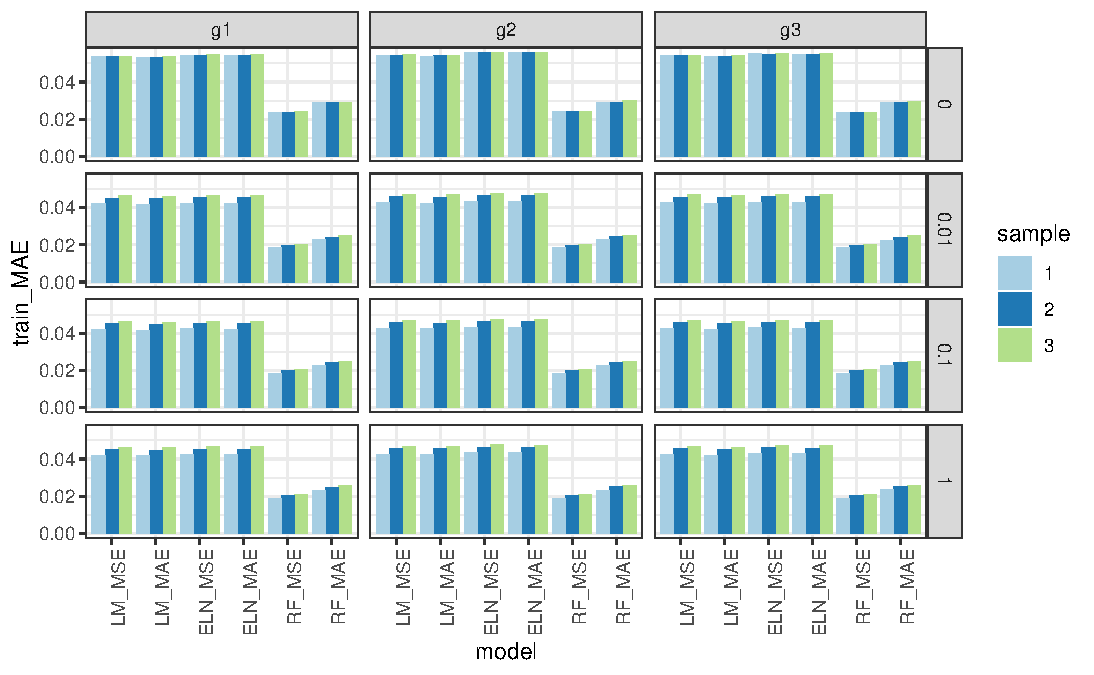
\includegraphics{simulation_train_mae.pdf}
	\caption{Simulation Train MAE}
\end{figure}

\begin{figure}
	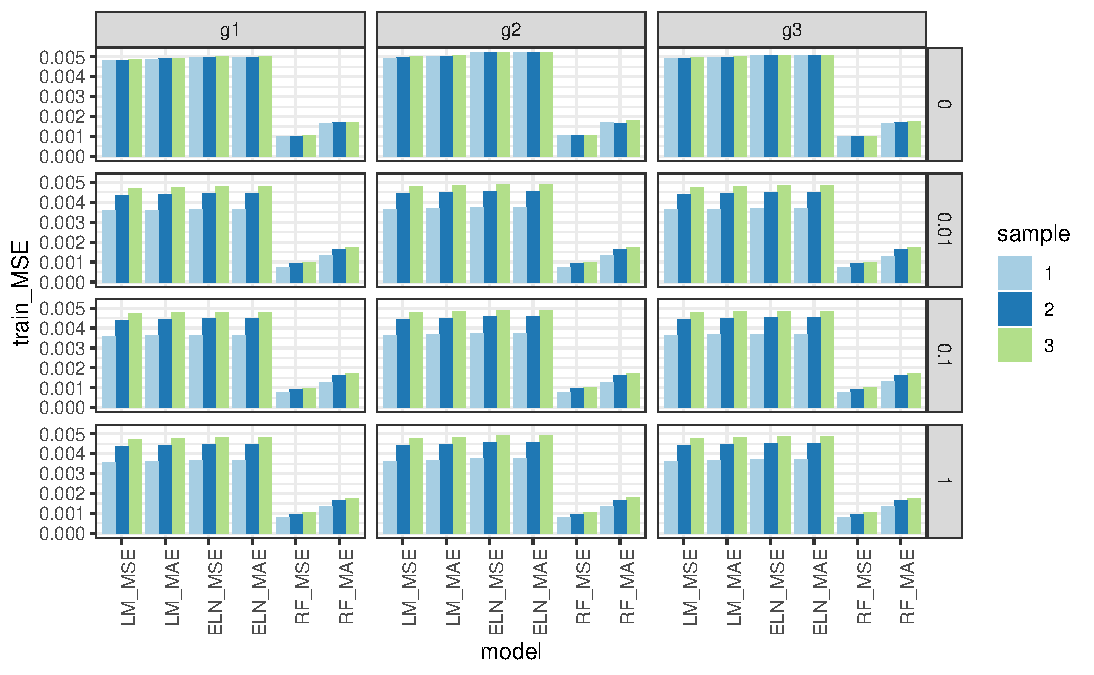
\includegraphics{simulation_train_mse.pdf}
	\caption{Simulation Train MSE}
\end{figure}

\begin{figure}
	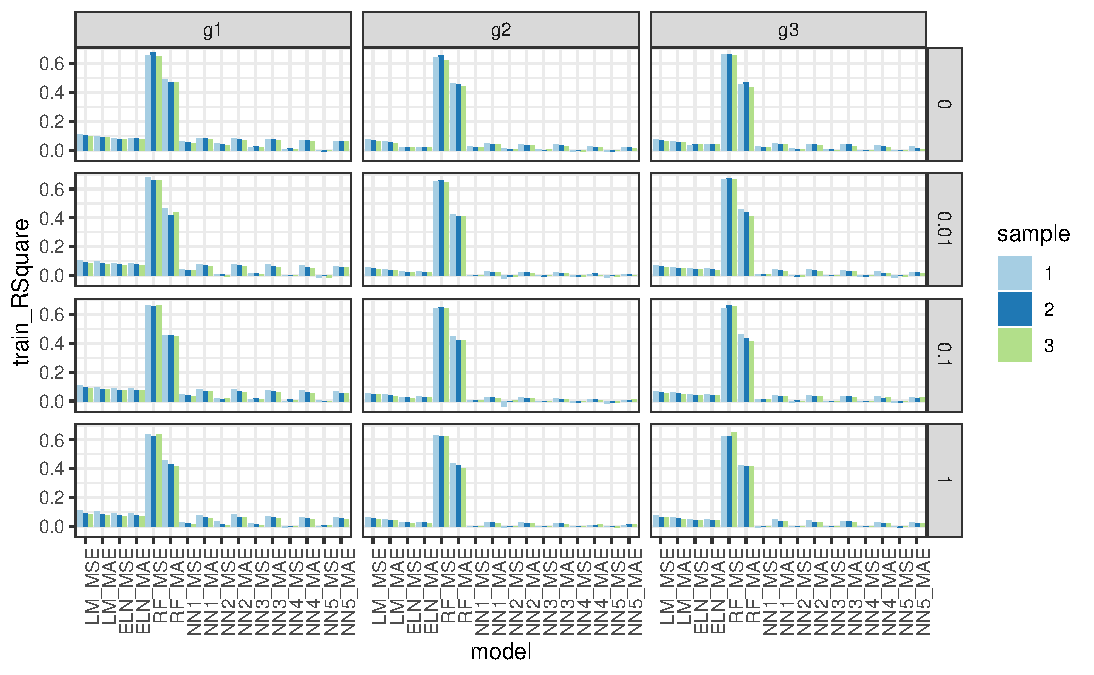
\includegraphics{simulation_train_rsquare.pdf}
	\caption{Simulation Train R Squared}
\end{figure}

\newpage

\subsubsection{Empirical Study}

\begin{figure}
	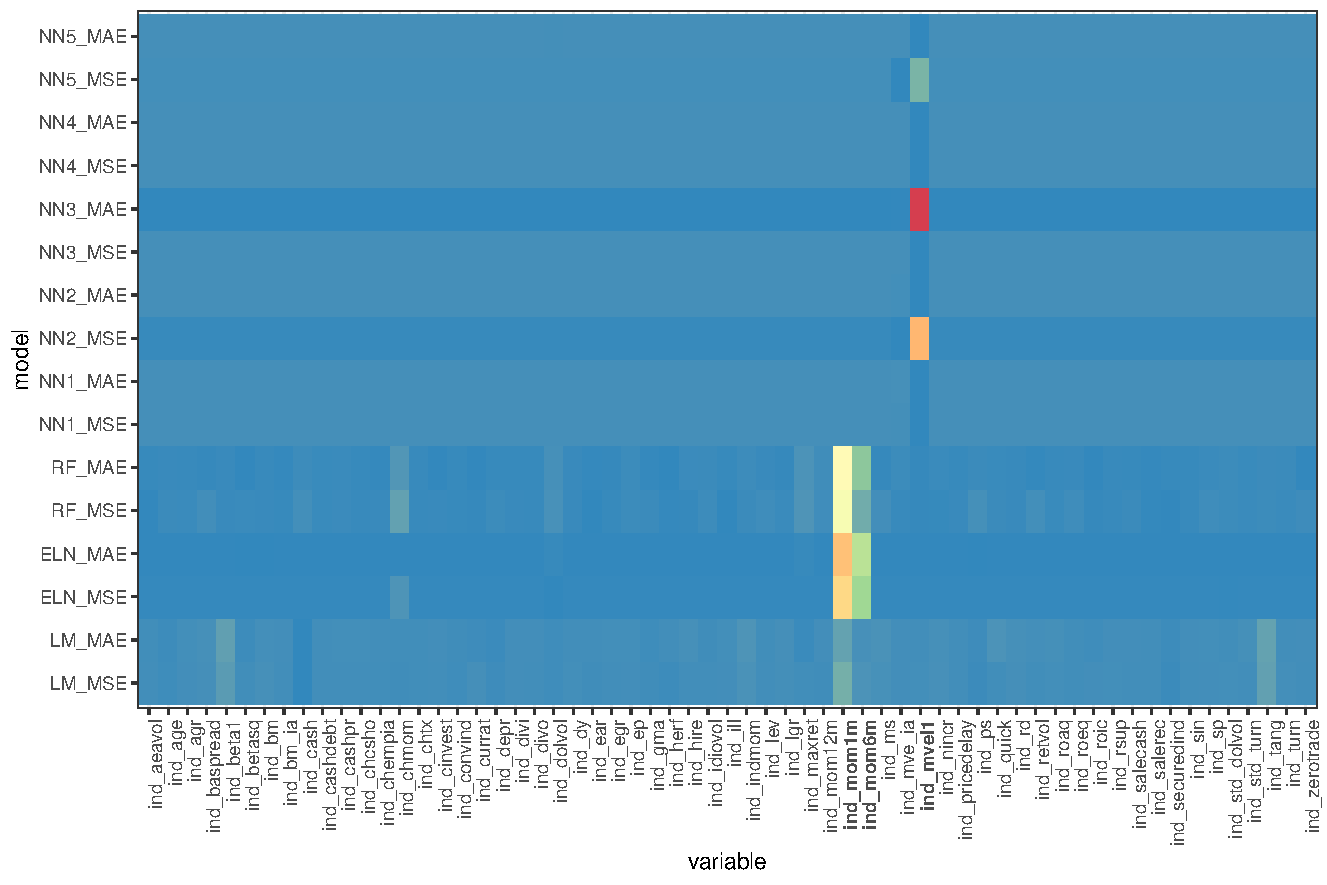
\includegraphics{empirical_sample_1_vi_ind.pdf}
	\caption{Empirical Data Individual Factor Variable Importance for Sample 1}
\end{figure}

\begin{figure}
	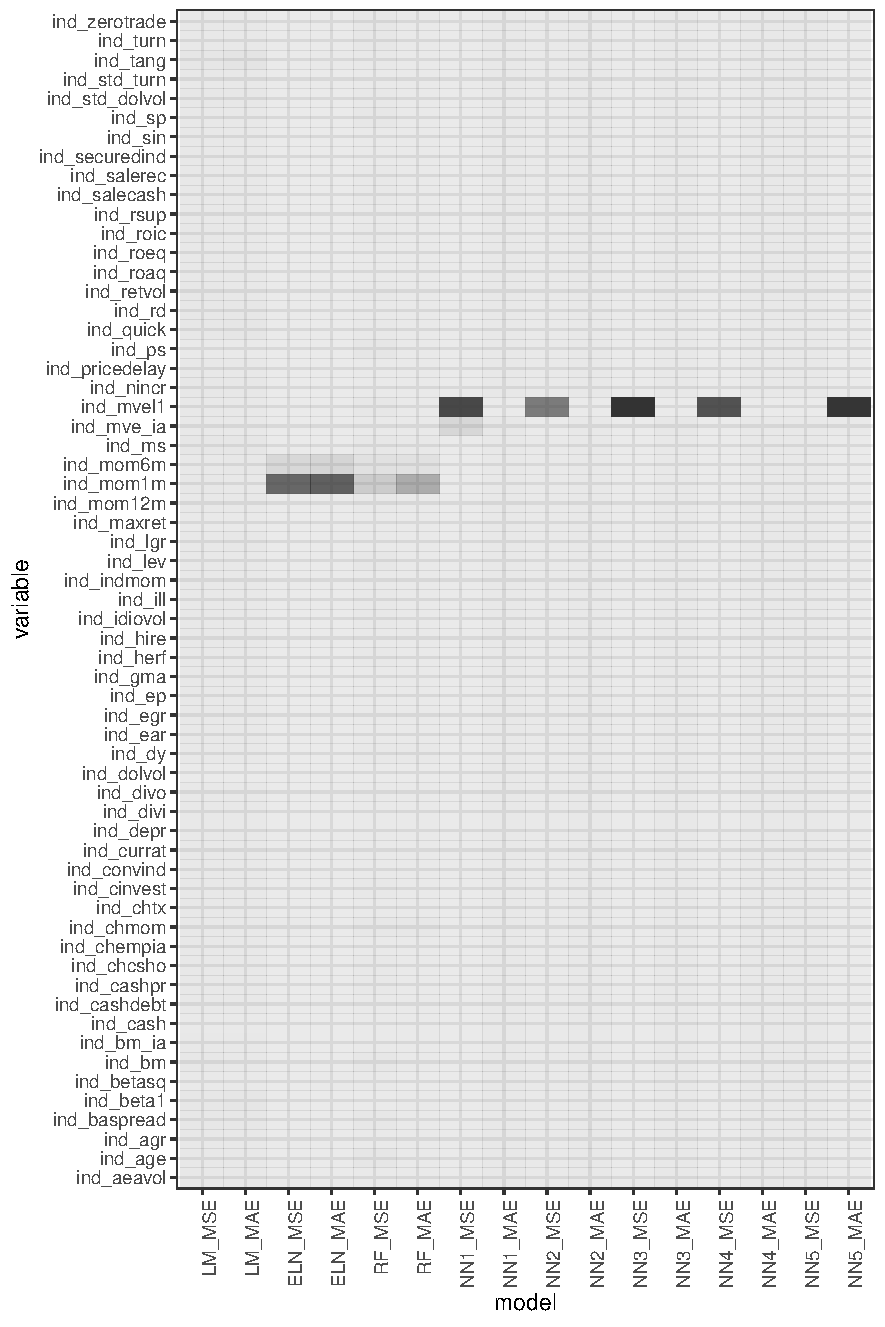
\includegraphics{empirical_sample_2_vi_ind.pdf}
	\caption{Empirical Data Individual Factor Variable Importance for Sample 2}
\end{figure}

\begin{figure}
	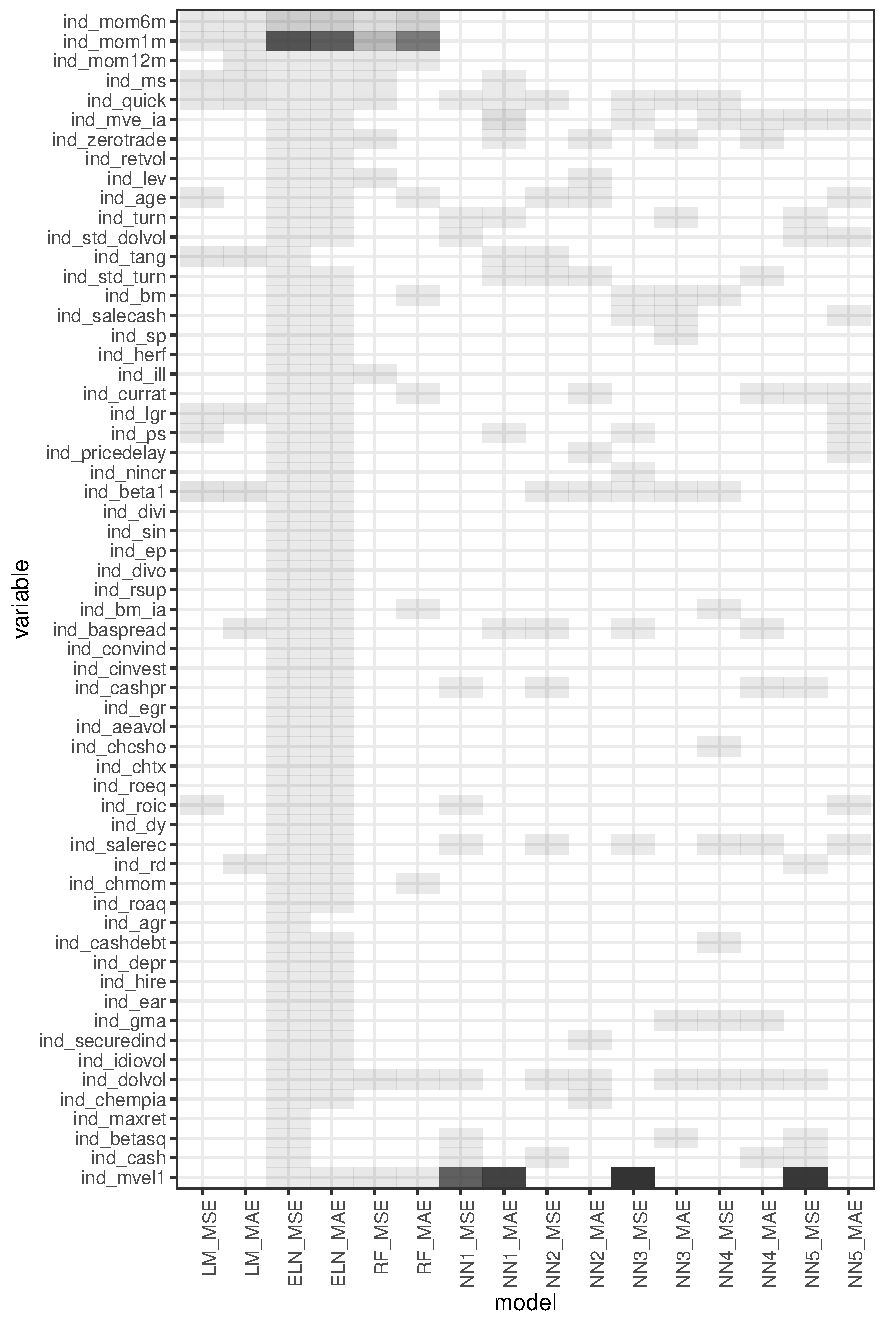
\includegraphics{empirical_sample_3_vi_ind.pdf}
	\caption{Empirical Data Individual Factor Variable Importance for Sample 3}
\end{figure}

\label{computation}

\newpage

\subsection{Computational Details}

\subsubsection{Linear Models}

OLS used for fitting wrt MSE.

quantreg package used for fitting wrt MAE. (minimizing 0.5 quantile loss is equivalent to minimizing mae).

\subsubsection{Penalized Linear}

The package \textbf{hqreg} was used to fit penalized regression models with respect to MSE and MAE.

This package efficiently calculates a regularization path of penalization values given a value for $\alpha$. This means that it is much more efficient to instead only supply a grid for $\alpha$, let the algorithm decide its own path of penalization values. The combination of these two parameters which produces the best results on the validation set were then chosen. Note that this is the approach originally suggested by \cite{zou_regularization_2005}.

\subsubsection{Classification and Regression Trees}

For full details of the Classification and Regression Tree algorithm see \cite{breiman_classification_1984}. 

\begin{algorithm}[H]
	\SetAlgoLined
	Initialize \;
	\For{$d$ from 1 to $L$}{
		\For{$i$ in ${C_l(d-1), l = 1, \dots, 2^{d-1}}$}{
			For each feature $j = 1, 2, \dots, P,$ and each threshold level $\alpha$, define a split as $s = (j, \alpha)$ which divides $C_l(d-1)$ into $C_{left}$ and $C_{right}$:
			\begin{equation*}
				C_{left}s = \{z_j \leq \alpha\} \cap C_l(d-1); C_{right}s = \{z_j > \alpha\} \cap C_l(d-1)
			\end{equation*}
			
			Define the impurity function:
			\begin{equation*}
				\mathcal{L}(C, C_{left}, C_{right}) = \frac{|C_{left}|}{|C|}H(C_{left}) + \frac{|C_{right}|}{|C|}H(C_{right})
			\end{equation*}
			where
			\begin{equation*}
			H(C) = \frac{1}{|C|} \sum_{ }^{z_{i,t}\in C}(r_{i,t+1}-\theta)^2, \theta = \frac{1}{|C|} \sum_{z_{i,t}\in C}^{ }r_{i,t+1}
			\end{equation*}
			and $|C|$ denotes the number of observations in set C
			
			Find the optimal split
			\begin{equation*}
				s^* \leftarrow \underset{s}{argmin}\mathcal{L}(C(s),C_{left}(s),C_{right}(s))
			\end{equation*}
			Update nodes (partition the data):
			\begin{equation*}
				C_{2l-1}(d) \leftarrow C_{left}(s^*), C_{2l}(d) \leftarrow C_{right}(s^*)
			\end{equation*}
		}
	}
	\KwResult{The prediction of a regression tree is:
	\begin{equation*}
		g(z_{i,t};\theta,L) = \sum_{k=1}^{2^L}\theta_k\textbf{1}_{z_{i,t}\in C_k(L)}; \theta_k = \frac{1}{|C_{k}(L)|} \sum_{z_{i,t}\in C_k(L)}^{ }r_{i,t+1}
	\end{equation*}
	}
	\caption{Classification and Regression Tree}
\end{algorithm}

\subsubsection{Random Forest}

The \textbf{randomforestSRC} package was used to fit both random forests for mean regression and quantile regression.

To maintain computational feasibility, all random forest models were grown using 50 trees, and their \textit{mtry} \textit{nodesize} hyperparameters tuned. 

Rather than use the randomly determined out of bag (OOB) observations for hyperparameter tuning, we explicitly use a separate validation set that is closer to the test set in time, in order to maintain temporal ordering of the data.

For full details of the Random Forest algorithm see \cite{breiman_random_2001}. 

\begin{algorithm}[H]
	\SetAlgoLined
	\For{$b$ from $1$ to $B$}{
		Draw bootstrap samples {$(z_{i,t},r_{i,t+1}),(i,t) \in Bootstrap(b)$} from the dataset\
		Grow a tree $T_b$ using Algorithm, using only a random subsample, say $\sqrt{P}$ of all features \
		Denote the resulting $bth$ tree as
		\begin{equation*}
			\hat{g}_b (z_{i,t},\hat{\theta}_b, L) = \sum_{k=1}^{2^L}\theta_b^k\textbf{1}_{z_{i,t}\in C_k(L)}
		\end{equation*}
	}
	\KwResult{The final random forest prediction is given by the output of all trees:
		\begin{equation*}
			\hat{g}_b (z_{i,t}; L, B) = \frac{1}{B} \sum_{b=1}^B \hat{g}_b (z_{i,t},\hat{\theta}_b, L)
		\end{equation*}
	}
	\caption{Random Forest}
\end{algorithm}

\subsubsection{Neural Networks}

Nueral Networks were fit using the \textbf{keras} package, using the \textbf{tensorflow} backend. 

Due to computational limitations, a systematic grid search or random search approach for hyperparameters was not feasible. Instead, common hyperparameters that are usually grid searched were tuned manually. 

\begin{table}
	\begin{tabular}{|lll|}
		\hline
		Hyperparameter & Options Considered & Optimal Choice \\ \hline
		Activation Function & ReLU, Leaky ReLU with $\alpha = (0.01, 0.1)$, tanh & tanh \\
		Optimizer & ADAM, NADAM & ADAM \\
		Learning Rate & (0.1, 0.01, 0.001, 0.0001) & 0.01 \\
		L1 Penalty & (1, 0.1, 0.01) & 0.01 \\
		Batch Size & (32, 64, 128, 256, 512, 1024, 2048, 4096) & 256 (Empirical), 128 (Simulated) \\
		Early Stopping Patience & (10, 20, 30, 40, 50) & 40 \\ \hline
	\end{tabular}
	\caption{Hyperparameters Considered for Neural Networks}
\end{table}



ADAM algorithm for stochastic gradient descent and learning rate shrinkage as detailed by \cite{kingma_adam:_2014}.

\begin{algorithm}
	\SetAlgoLined
	Initialize $j = 0$, $\epsilon = \infty$ and select the patience parameter $p$ (max iterations)\
	
	\While{j < p}{
		Update $\theta$ using the training algorithm\
		Calculate the prediction error from the validation sample, denoted as \(\epsilon'\)\
		
		\eIf{\(\epsilon' < \epsilon\)}
			{\(j \leftarrow 0\)\
				
			 \(\epsilon \leftarrow \epsilon'\)\
			 
		     \(\theta' \leftarrow \theta\)}
	     	{\(j \leftarrow j+1\)}
	}
	\KwResult{$\theta'$ is the final parameter estimate}
	\caption{Early stopping via validation}
\end{algorithm}

Batch Normalization Algorithm as detailed by \cite{ioffe_batch_2015}.

\begin{algorithm}
	Input: Values of \(x\) for each activation over a batch \(\mathcal{B} = {x_1, x_2, \dots, x_N}\)
	
	\(\mu_\mathcal{B} \leftarrow \frac{1}{N} \sum_{i = 1}^{N}x_i\)
	
	\(\sigma_\mathcal{B}^2 \leftarrow \frac{1}{N} \sum_{i = 1}^{N}(x_i - \mu_\mathcal{B})^2\)
	
	\(\hat{x_i} \leftarrow \frac{x_i - \mu_\mathcal{B}}{\sqrt{\sigma_\mathcal{B}^2 + \epsilon}}\)
	
	\(y_i \leftarrow \gamma\hat{x_i} + \beta := BN_{\gamma, \beta}(x_i)\)
	
	\KwResult{\(y_i = BN_{\gamma, \beta}(x_i) : i = 1, 2, ..., N\)}
	\caption{Batch Normalization for one activation over one batch}
\end{algorithm}

\subsubsection{Tuning of Simulated Datasets}

The simulated datasets were tuned according to the following statistics: average individual time series R squared, average annualized volatility, and cross sectional R squared, and true/predictive R squared.

The methodology for evaluating average time series R squared and cross sectional R squared is consistent with that detailed by \cite{cochrane_asset_2005}. The steps are reproduced here for reference; for complete details refer to \cite{cochrane_asset_2005}.

First evaluate the following OLS model:

\begin{equation}
	R_{it} = a_i + \beta_i' f_{it} + \epsilon_{it} 
\end{equation}

where $f_{it}$ represents the \textit{true} factors in the returns process. The corresponding R-squared value for this time series regression is calculated across all stocks and averaged to yield the average time series R-Squared. 

A cross sectional regression for the risk premia is then run across assets of average returns on the factor coefficients:

\begin{equation}
	\bar{R_{it}} = \alpha_i = \beta_i' \lambda
\end{equation}

where the $\beta_i'$ are the estimated coefficients from each time series regressions run previously. The corresponding R squared for this regression is the cross sectional R squared.

The true R squared is a measure of signal to noise ratio i.e. how much of the returns data is due to 
This is simply calculated by running a pooled ordinary least squares regression on the entire panel, using the underlying g() as the "predictions.' The resulting R squared value is therefore a measure of how much of the panel can be explained by the g() term exclusive of any noise or error terms.

%%%%%%%%%%%%%%%%%%%%%%%%%%%%%%%%%%
%%BIBLIOGRAPHY
%%%%%%%%%%%%%%%%%%%%%%%%%%%%%%%%%%

\bibliographystyle{jfe}
\bibliography{Bibliography}

\end{document}